This Online Appendix presents the results of various empirical analyses that confirm the robustness of our analyses to different specifications, samples, and measures of crime. First, we show that the effects of the program on arrests and reported crimes from administrative records are not driven by the inclusion of a broader sample of municipalities in this dataset. Second, we show that our findings are robust to the use of alternative difference-in-differences estimators for staggered treatment adoption. Third, we show that the estimates presented in the main body of the paper are very similar to the ones we obtain using a balanced panel of municipalities. Fourth, we show that the results for reported crime and arrests are very similar when we use the full set of post-treatment and pre-treatment periods instead of capping the event study for symmetry with the ENUSC-based analysis. Fifth, we show that our main results remain statistically significant after applying a Bonferroni correction for multiple hypothesis testing. Sixth, we show that the results are not driven by broader temporal trends unrelated to police presence, using a placebo test based on non-neighborhood crime. Seventh, we establish that the effects of the program on crime perception remain consistent when alternative measures of crime perception available in the dataset are used. Eighth, we show that our results are robust to excluding municipalities most affected by the 2010 Maule earthquake. Finally, we document that \emph{Plan Cuadrante} has limited effects on neighboring municipalities, making it unlikely that the program’s impact on crime victimization is biased due to crime displacement.

\subsection{Effects of \emph{Plan Cuadrante} Using Administrative Data and the Sample of Municipalities Included in the ENUSC Survey}

The results reported in panel (b) of Figure \ref{fig:figure02} and in panel (a) of Figure \ref{fig:effectiveness_es} in the main manuscript show the effects of \emph{Plan Cuadrante} on the number of reported crimes in the municipality and the total number of arrests, which are administrative data provided by the police for all Chilean municipalities. The latter analysis is conducted with all never treated municipalities and municipalities that implemented the program between 2003 and 2013. This is a different analytical sample from the one used in the analysis of ENUSC survey outcomes -victimization, trust in the police, crime perception, and crime prevention measures- since the ENUSC survey was conducted only on a subsample of municipalities and for a different time period.

In this Online Appendix, we estimate the effects of \emph{Plan Cuadrante} on the number of crimes reported to the police and on the total number of arrests, using only the subsample of municipalities included in the analysis of the ENUSC outcomes. The sample size in this analysis is smaller, and the results are reported in Figure \ref{fig:figure02_N47}. While the effects for reported crime are larger in magnitude, the estimates are qualitatively similar to those observed in Table \ref{tab:SPD_all_vs_enusc} with the full sample. The estimated effect on arrests, however, is not statistically significant in this smaller ENUSC subsample, likely reflecting reduced power given the smaller number of municipalities and observations.




\begin{table}[h!]
\caption{Effects of \emph{Plan Cuadrante} on Reported Crime and Arrests: Full Sample and ENUSC Municipalities}
\label{tab:SPD_all_vs_enusc}
\begin{center}
\resizebox{12cm}{!}{
\begin{tabular}{lccccccccccccccccccccccccccccccccccccccc} \hline \hline
& & (1) & (2) & (3) & (4) \\
Outcome & & \multicolumn{2}{c}{Reported crime} & \multicolumn{2}{c}{Arrests} \\
\cmidrule(lr){3-4} \cmidrule(lr){5-6}
& & \shortstack{Sample\\Admin} & \shortstack{Sample\\ENUSC} & \shortstack{Sample\\Admin} & \shortstack{Sample\\ENUSC} \\
\cmidrule(lr){3-4} \cmidrule(lr){5-6}
\\
ATT & & -208.02*** & -428.09*** & 48.02*** & 44.09 \\
& & (56.13) & (108.48) & (16.27) & (34.85) \\
\\
N & & 4,231 & 592 & 3,293 & 405 \\
Municipalities & & 292 & 47 & 281 & 40 \\
Y mean & & 2,109.64 & 2,294.96 & 345.65 & 419.61 \\
\hline \hline
\end{tabular}}
\par{
\begin{tabular}{p{12cm}}
\footnotesize{Note: This table shows the effects of \emph{Plan Cuadrante} on the number of crimes reported to the police in the municipality per 100,000 inhabitants and on the number of arrests in the municipality per 100,000 inhabitants using administrative data from the Undersecretary for Crime Prevention. The table reports the results for two samples: the full sample of municipalities included in the administrative database that is used for the analysis of these outcomes and the subsample of these municipalities included in the analysis of ENUSC outcomes. The estimation is conducted using the procedure developed in \citet{Callaway} for difference-in-differences with staggered treatment adoption. Standard errors are clustered at the municipality level using the wild bootstrapping procedure. ***p$<$0.01, **p$<$0.05, *p$<$0.1.} \\
\end{tabular}}
\end{center}
\end{table}

\clearpage
%--- Implementation
\begin{figure}[h!]
    \centering
    \caption{Effects of \emph{Plan Cuadrante} on Reported Crime and Arrests (Sample of Municipalities Included in the Analysis of ENUSC Outcomes)}
    \label{fig:figure02_N47}
    \begin{subfigure}{0.495\textwidth}
        \centering
        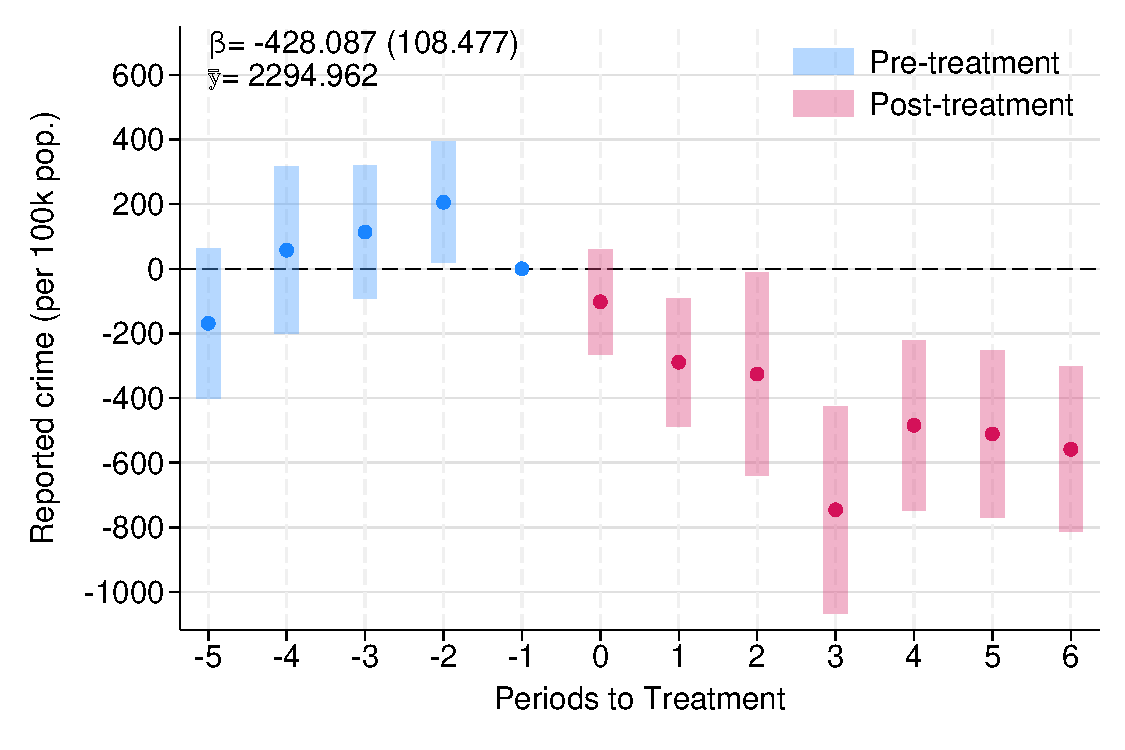
\includegraphics[width=\textwidth]{../manuscript/Graphs/totalreportedcrime_47enusc.pdf}
        \caption{Reported crime per 100k inhabitants}
    \end{subfigure}%
    ~ 
    \begin{subfigure}{0.495\textwidth}
    \centering
    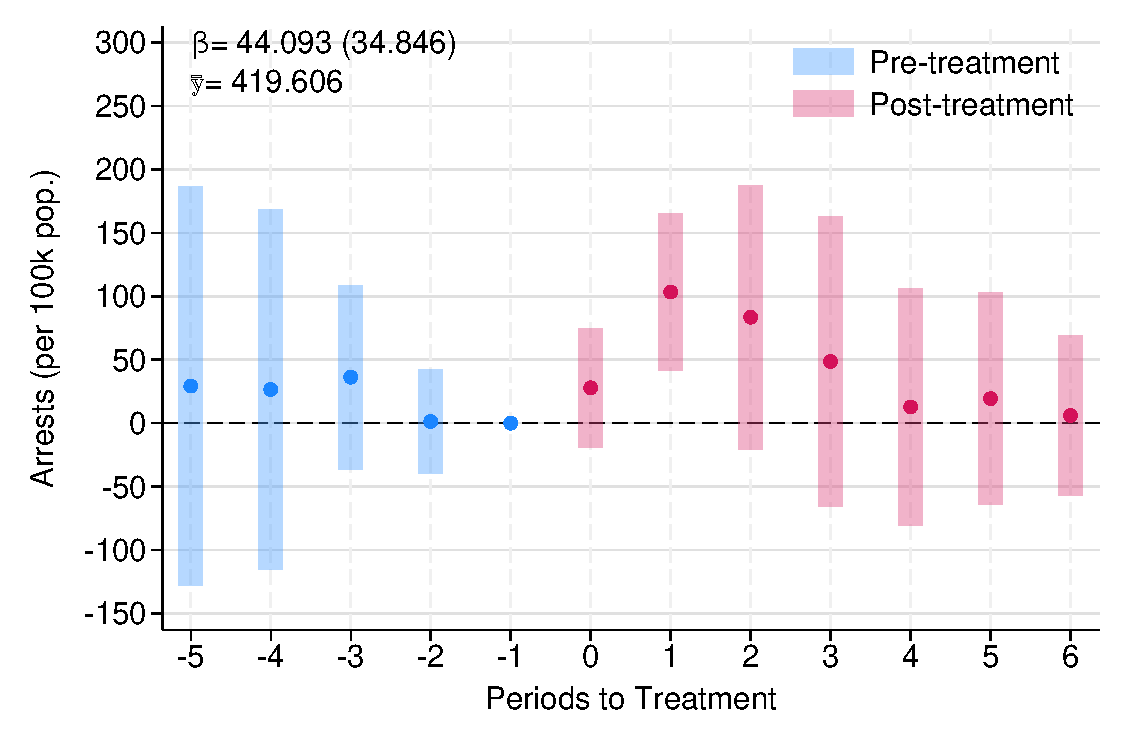
\includegraphics[width=\textwidth]{../manuscript/Graphs/totalarrestscrime_47enusc.pdf}
        \caption{Arrests per 100k inhabitants}
    \end{subfigure}
    \\[12pt]
    \begin{minipage}{0.99\textwidth}
    \footnotesize Notes: This figure shows the dynamic effects of \emph{Plan Cuadrante} on the number of crimes reported to the police per 100,000 inhabitants in the municipality in panel (a) and on the number of arrests per 100,000 inhabitants in the municipality in panel (b) using administrative data from the Undersecretary for Crime Prevention. The analysis is conducted using only the sample of municipalities included in the analysis of ENUSC outcomes. Panel (a) includes 592 observations, while panel (b) includes 405 observations. The estimation is conducted using the procedure developed in \citet{Callaway} for difference-in-differences with staggered treatment adoption. The dots in the figure represent the estimated coefficients and the bars behind them 95\% confidence intervals. Standard errors are clustered at the municipality level using wild bootstrapping. The pooled effect and the mean outcome before the introduction of the treatment is also presented in each panel. 
    \end{minipage}
\end{figure}

\clearpage

\subsection{Alternative Estimation Methods}

The results reported in Section \ref{main_results} are estimated using the difference-in-differences estimator for staggered treatment adoption developed in \citet{Callaway}. In this subsection, we examine the robustness of the results to the use of alternative difference-in-difference estimators for staggered treatment adoption including those developed in \citet{Chaisemartin}, \citet{Gardner}, \citet{wooldridge2023simple}, and also to the canonical two-way fixed effects (TWFE). 

The results of these analyses are reported in Figure \ref{fig:figureA2_alterestim} and show similar effects of \emph{Plan Cuadrante} in terms of both magnitude and statistical significance across most specifications. On the other hand, the canonical TWFE shows smaller effects, likely due to the negative weights problem highlighted by \citet{GoodmanBacon} when estimating difference-in-differences with staggered treatment adoption using TWFE.


\begin{figure}[h!]
    \centering
    \caption[Effects of \emph{Plan Cuadrante} on Police Effectiveness Using Alternative Estimators]{Effects of \emph{Plan Cuadrante} on Police Effectiveness Using Alternative Estimators}
    \label{fig:figureA2_alterestim}
    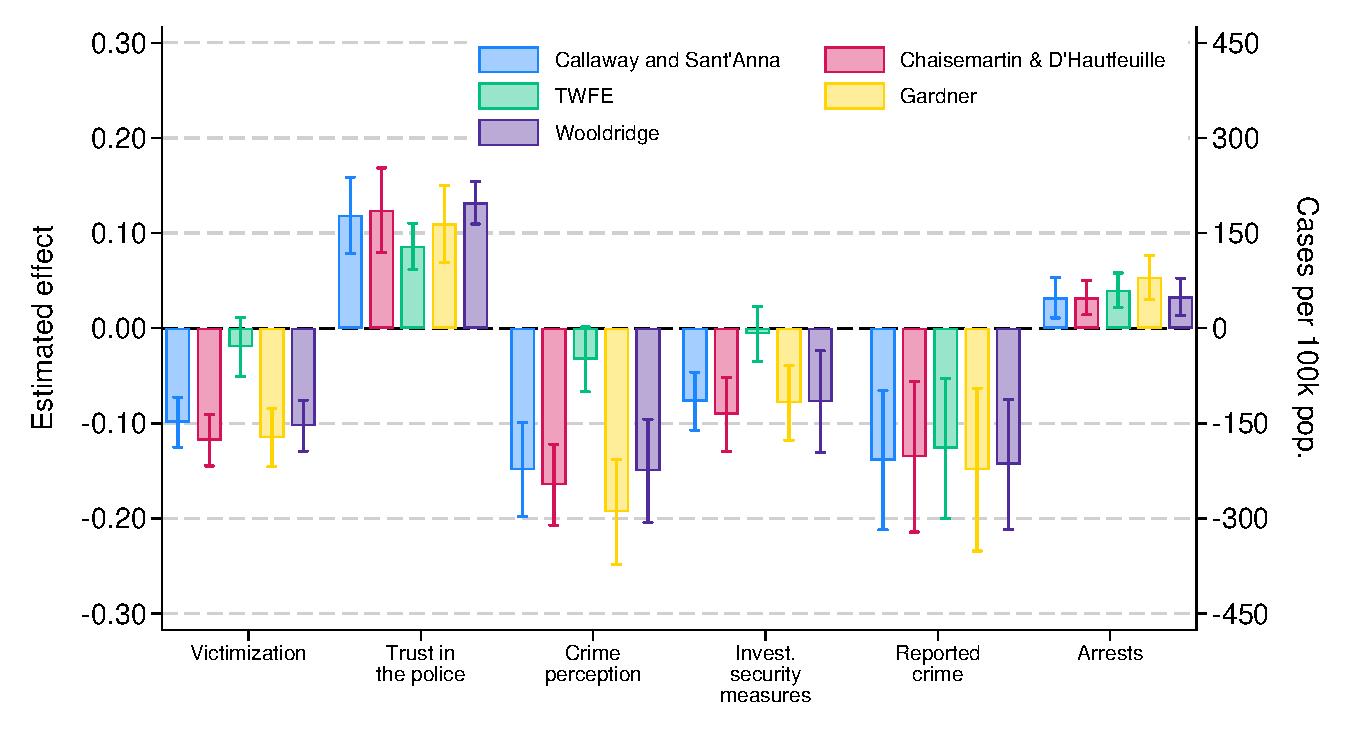
\includegraphics[width=\textwidth]{../manuscript/Graphs/Comparison_estimators_combined.pdf}
    \\[8pt]
    \begin{minipage}{0.99\textwidth}
    \footnotesize Notes: The figure reports the effects of \emph{Plan Cuadrante} on different measures of police effectiveness using various difference-in-differences estimators, including the methods developed in \citet{Callaway}, \citet{Chaisemartin}, \citet{Gardner}, \citet{wooldridge2023simple}, and the canonical two-way fixed effects (TWFE). Bars are the estimated post-treatment effects and the whiskers the 95\% confidence intervals; standard errors are clustered at the municipality level. Victimization is the probability of household victimization in the last 12 months; reported crime is the number of crimes reported to the police in the municipality per 100,000 inhabitants; crime perception is the probability of perceiving an increase in crime; investment in security measures is the probability of adopting security measures in the last twelve months; trust in the police is the probability of reporting high trust in the police; and arrests is the number of arrests per 100,000 inhabitants. Reported crime and arrests (administrative data) are read on the right axis; all other outcomes, from the ENUSC survey, are read on the left axis.
    \end{minipage}
\end{figure}


Figures \ref{fig:alterestim_delitos} through \ref{fig:alterestim_crime} report the corresponding event-study estimates for victimization, crime perception, investment in security measures, and reported crime under each alternative estimator. Pre-treatment coefficients are consistently small and statistically indistinguishable from zero across all estimators and outcomes, confirming that the parallel trends assumption holds regardless of the estimation method. Post-treatment effects remain negative and statistically significant across these outcomes, closely mirroring the results from the main specification in Figure \ref{fig:figure02}.

% =============================================================================
% Alternative-estimator robustness figures
% Each figure shows the event study from three estimators:
%   (a) Chaisemartin & D'Hautfeuille
%   (b) Gardner
%   (c) Wooldridge
% Callaway & Sant'Anna is excluded — it appears as the headline figure.
%
% First block (3 figures): ENUSC survey outcomes
% Second block (1 figure): SPD administrative crime outcomes
% =============================================================================


% ----- Victimization (delitos) -----------------------------------------------
\begin{figure}[h!]
    \centering
    \caption[Effects of \emph{Plan Cuadrante} on Victimization Using Alternative Estimators]{Effects of \emph{Plan Cuadrante} on Victimization Using Alternative Estimators}
    \label{fig:alterestim_delitos}
    \begin{subfigure}{0.47\textwidth}
        \centering
        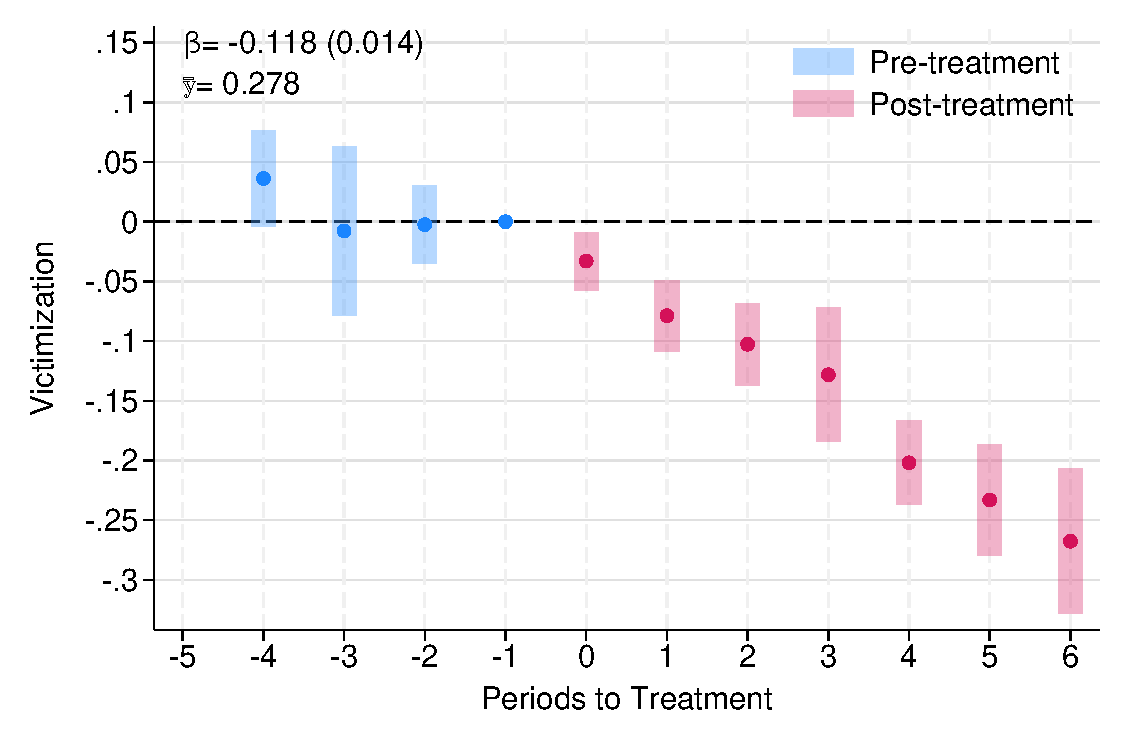
\includegraphics[width=\textwidth]{../manuscript/Graphs/CHDH_event_study_delitos.pdf}
        \caption{Chaisemartin \& D'Hautfeuille}
    \end{subfigure}%
    \begin{subfigure}{0.47\textwidth}
        \centering
        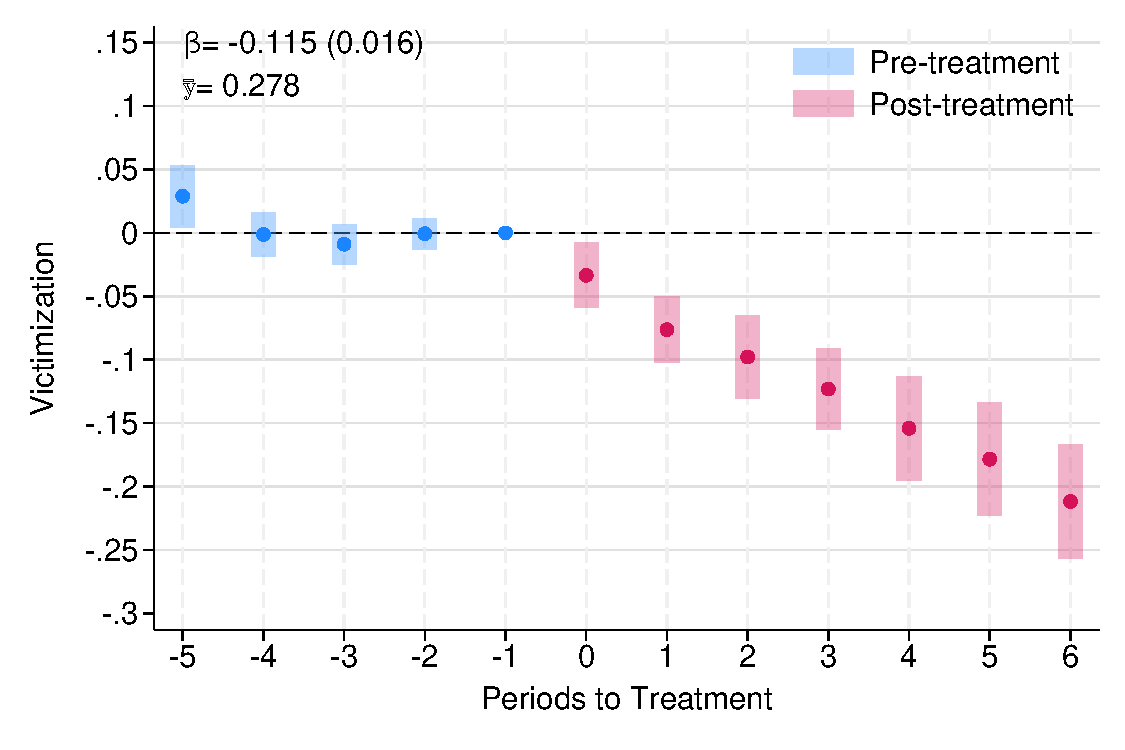
\includegraphics[width=\textwidth]{../manuscript/Graphs/DID2S_event_study_delitos.pdf}
        \caption{Gardner}
    \end{subfigure}
    \\[6pt]
    \begin{subfigure}{0.47\textwidth}
        \centering
        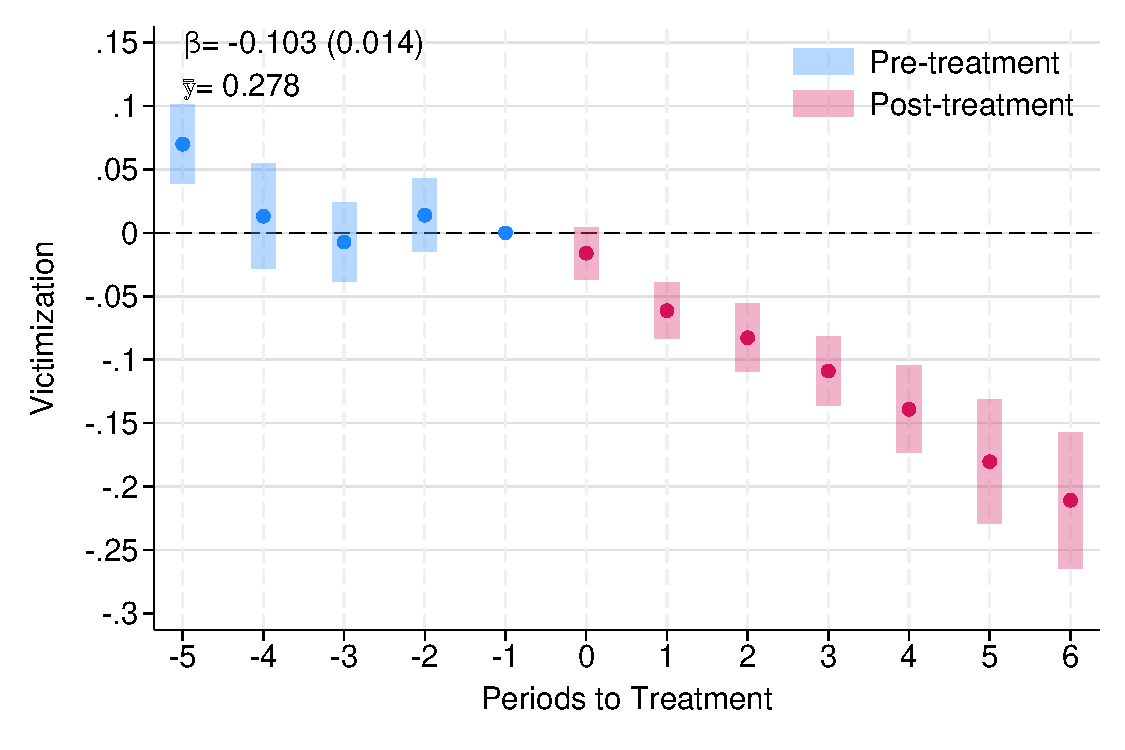
\includegraphics[width=\textwidth]{../manuscript/Graphs/JWDID_event_study_delitos.pdf}
        \caption{Wooldridge}
    \end{subfigure}
    \\[12pt]
    \begin{minipage}{0.99\textwidth}
    \footnotesize Notes: The figure reports event-study estimates of the effect of \emph{Plan Cuadrante} on the probability of household victimization in the last 12 months using the ENUSC survey, estimated with three alternative difference-in-differences estimators robust to staggered adoption: \citet{Chaisemartin} in panel (a), \citet{Gardner} in panel (b), and \citet{wooldridge2023simple} in panel (c). Each panel plots the estimated coefficient at each event time relative to treatment along with 95\% confidence intervals. Standard errors are clustered at the municipality level. The headline coefficient $\beta$ corresponds to the average post-treatment effect, and $\bar{y}$ denotes the never-treated mean of the outcome over the sample period.
    \end{minipage}
\end{figure}


% ----- Crime perception (inseguridad_barrio1) --------------------------------
\begin{figure}[h!]
    \centering
    \caption[Effects of \emph{Plan Cuadrante} on Crime Perception Using Alternative Estimators]{Effects of \emph{Plan Cuadrante} on Crime Perception Using Alternative Estimators}
    \label{fig:alterestim_inseguridad}
    \begin{subfigure}{0.47\textwidth}
        \centering
        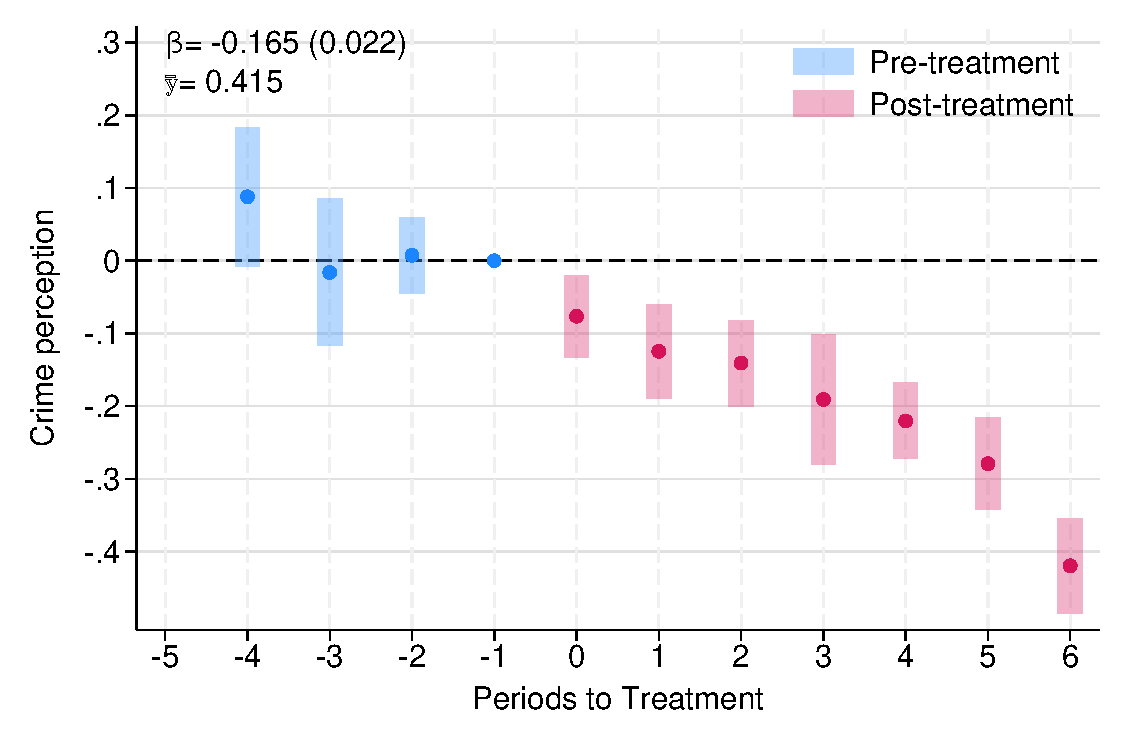
\includegraphics[width=\textwidth]{../manuscript/Graphs/CHDH_event_study_inseguridad_barrio1.pdf}
        \caption{Chaisemartin \& D'Hautfeuille}
    \end{subfigure}%
    \begin{subfigure}{0.47\textwidth}
        \centering
        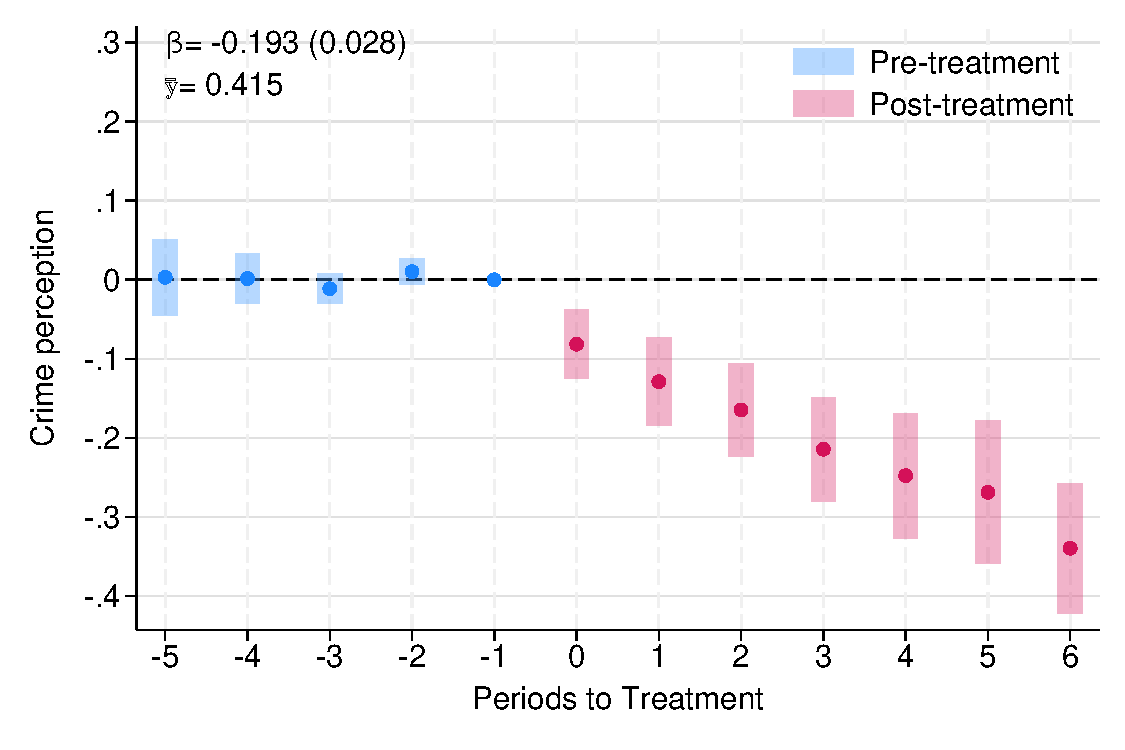
\includegraphics[width=\textwidth]{../manuscript/Graphs/DID2S_event_study_inseguridad_barrio1.pdf}
        \caption{Gardner}
    \end{subfigure}
    \\[6pt]
    \begin{subfigure}{0.47\textwidth}
        \centering
        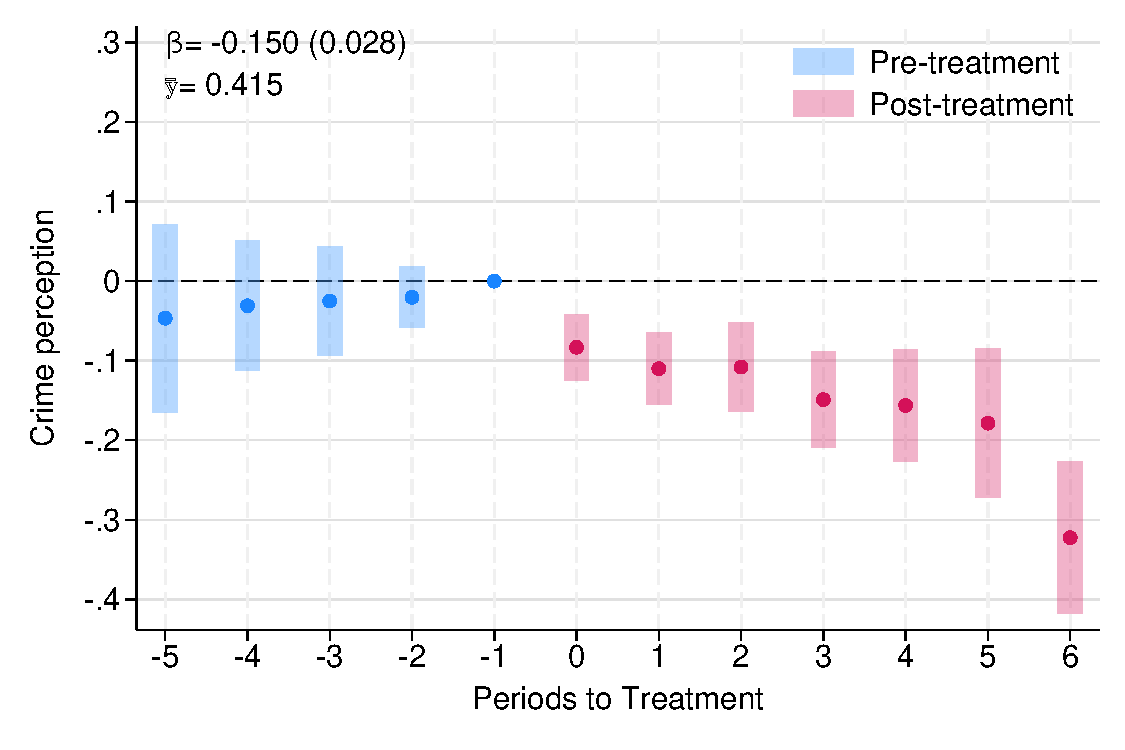
\includegraphics[width=\textwidth]{../manuscript/Graphs/JWDID_event_study_inseguridad_barrio1.pdf}
        \caption{Wooldridge}
    \end{subfigure}
    \\[12pt]
    \begin{minipage}{0.99\textwidth}
    \footnotesize Notes: The figure reports event-study estimates of the effect of \emph{Plan Cuadrante} on the probability of perceiving an increase in crime using the ENUSC survey, estimated with three alternative difference-in-differences estimators robust to staggered adoption: \citet{Chaisemartin} in panel (a), \citet{Gardner} in panel (b), and \citet{wooldridge2023simple} in panel (c). Each panel plots the estimated coefficient at each event time relative to treatment along with 95\% confidence intervals. Standard errors are clustered at the municipality level. The headline coefficient $\beta$ corresponds to the average post-treatment effect, and $\bar{y}$ denotes the never-treated mean of the outcome over the sample period.
    \end{minipage}
\end{figure}


% ----- Private investment in security (medidas_general_12) -------------------
\begin{figure}[h!]
    \centering
    \caption[Effects of \emph{Plan Cuadrante} on Investment in Security Measures Using Alternative Estimators]{Effects of \emph{Plan Cuadrante} on Investment in Security Measures Using Alternative Estimators}
    \label{fig:alterestim_medidas}
    \begin{subfigure}{0.47\textwidth}
        \centering
        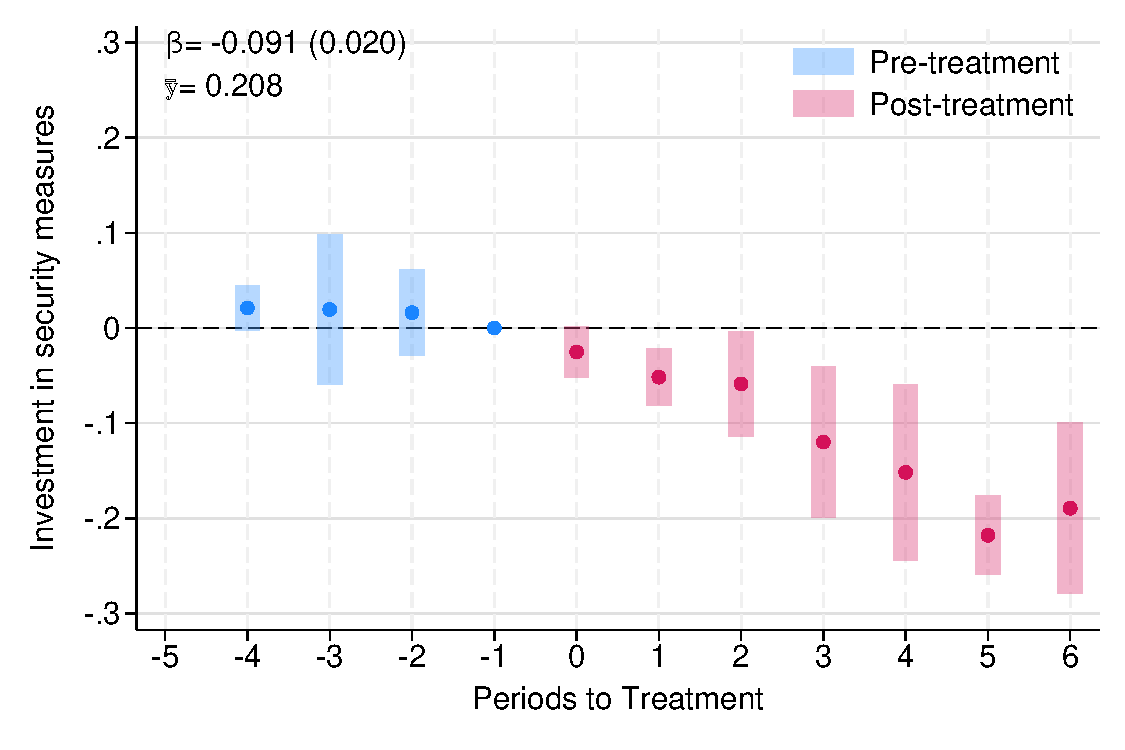
\includegraphics[width=\textwidth]{../manuscript/Graphs/CHDH_event_study_medidas_general_12.pdf}
        \caption{Chaisemartin \& D'Hautfeuille}
    \end{subfigure}%
    \begin{subfigure}{0.47\textwidth}
        \centering
        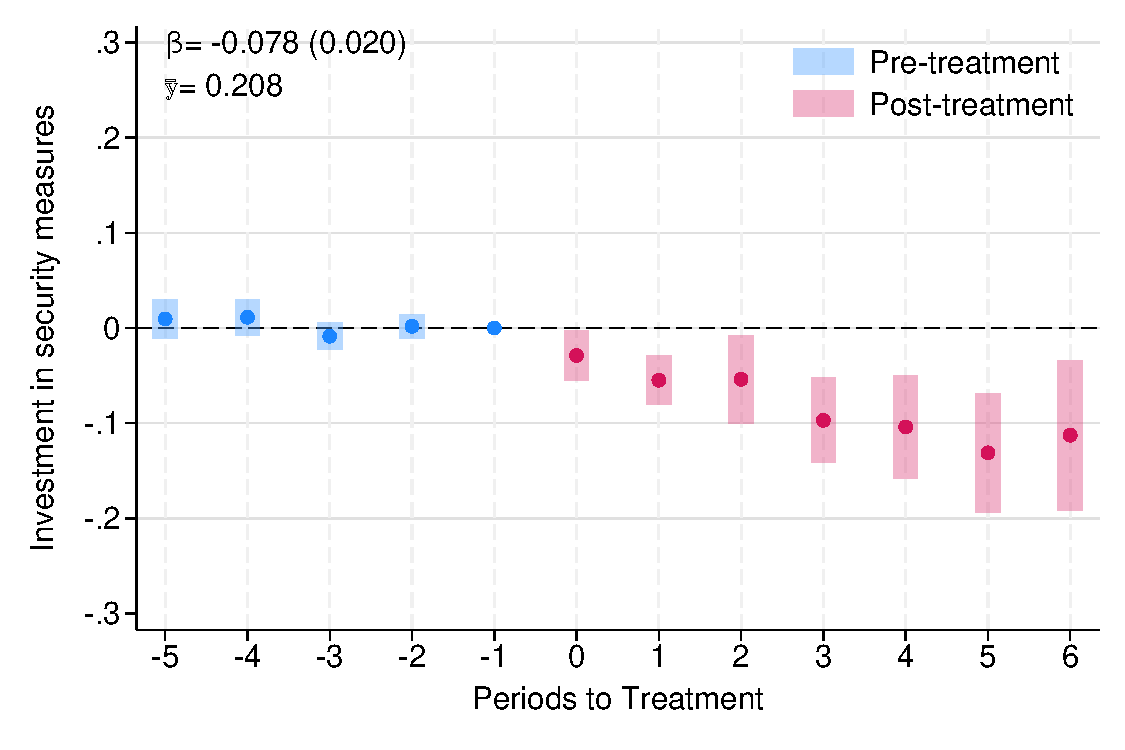
\includegraphics[width=\textwidth]{../manuscript/Graphs/DID2S_event_study_medidas_general_12.pdf}
        \caption{Gardner}
    \end{subfigure}
    \\[6pt]
    \begin{subfigure}{0.47\textwidth}
        \centering
        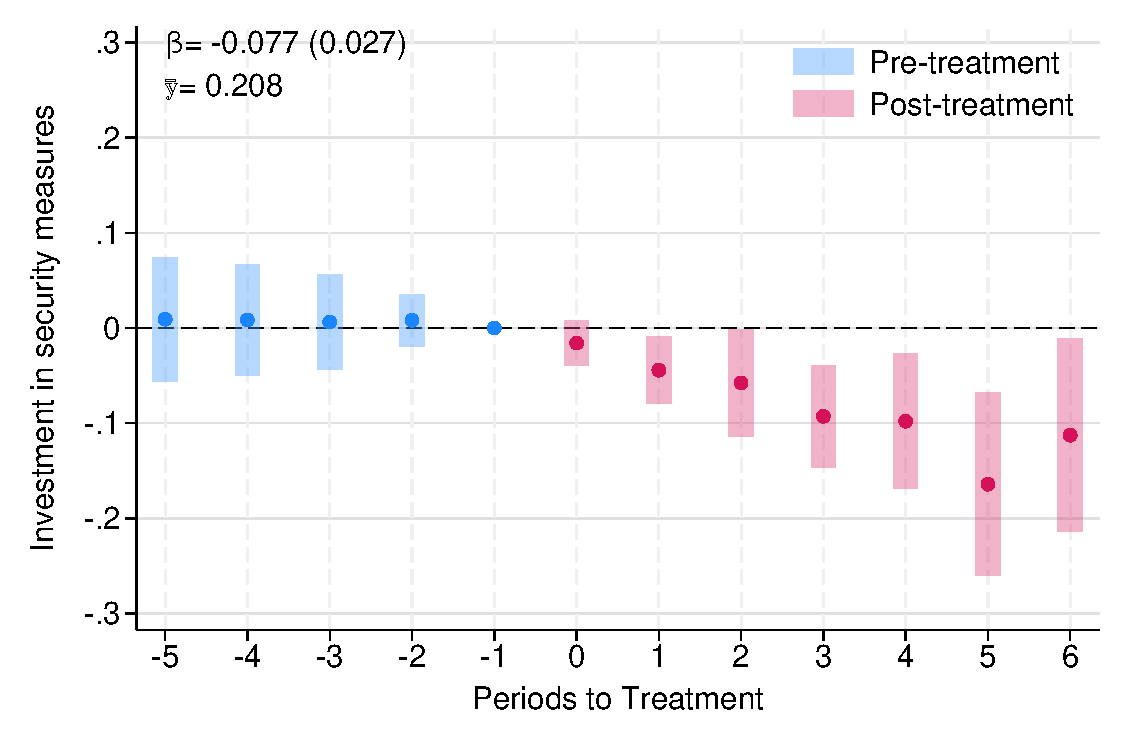
\includegraphics[width=\textwidth]{../manuscript/Graphs/JWDID_event_study_medidas_general_12.pdf}
        \caption{Wooldridge}
    \end{subfigure}
    \\[12pt]
    \begin{minipage}{0.99\textwidth}
    \footnotesize Notes: The figure reports event-study estimates of the effect of \emph{Plan Cuadrante} on the probability of adopting security measures in the last twelve months using the ENUSC survey, estimated with three alternative difference-in-differences estimators robust to staggered adoption: \citet{Chaisemartin} in panel (a), \citet{Gardner} in panel (b), and \citet{wooldridge2023simple} in panel (c). Each panel plots the estimated coefficient at each event time relative to treatment along with 95\% confidence intervals. Standard errors are clustered at the municipality level. The headline coefficient $\beta$ corresponds to the average post-treatment effect, and $\bar{y}$ denotes the never-treated mean of the outcome over the sample period.
    \end{minipage}
\end{figure}


% =============================================================================
% Administrative data (SPD municipality-level)
% =============================================================================


% ----- Reported crime --------------------------------------------------------
\begin{figure}[h!]
    \centering
    \caption[Effects of \emph{Plan Cuadrante} on Reported Crime Using Alternative Estimators]{Effects of \emph{Plan Cuadrante} on Reported Crime Using Alternative Estimators}
    \label{fig:alterestim_crime}
    \begin{subfigure}{0.47\textwidth}
        \centering
        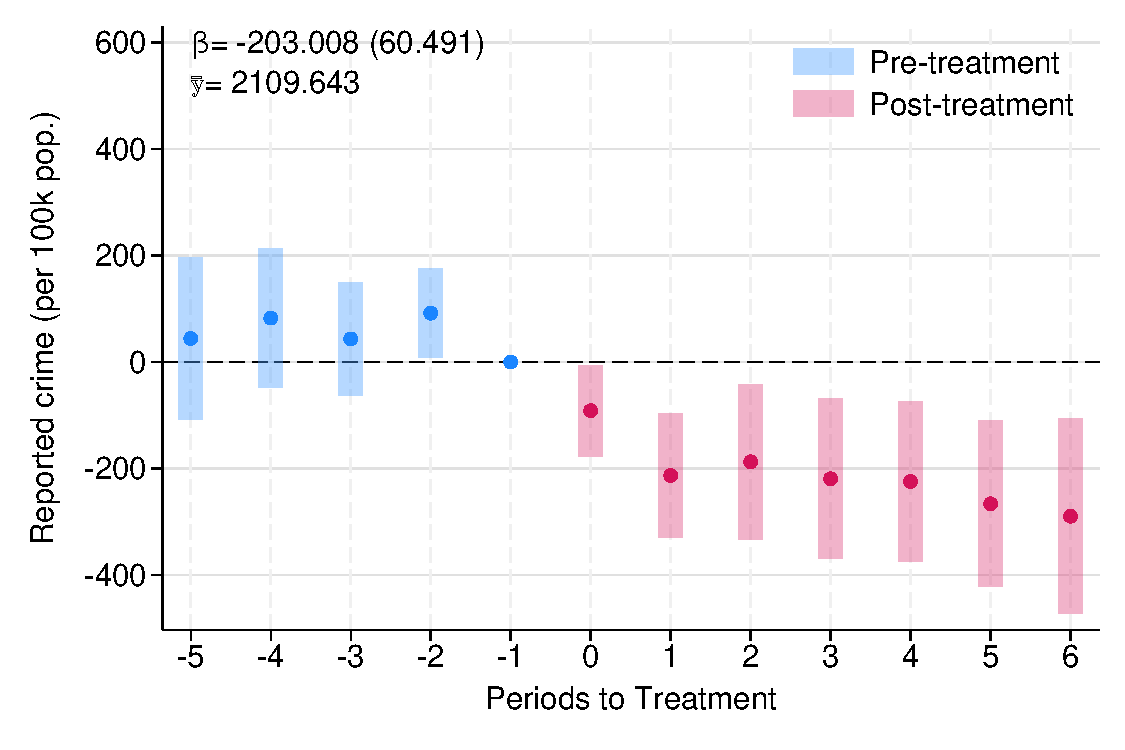
\includegraphics[width=\textwidth]{../manuscript/Graphs/CHDH_event_study_crime.pdf}
        \caption{Chaisemartin \& D'Hautfeuille}
    \end{subfigure}%
    \begin{subfigure}{0.47\textwidth}
        \centering
        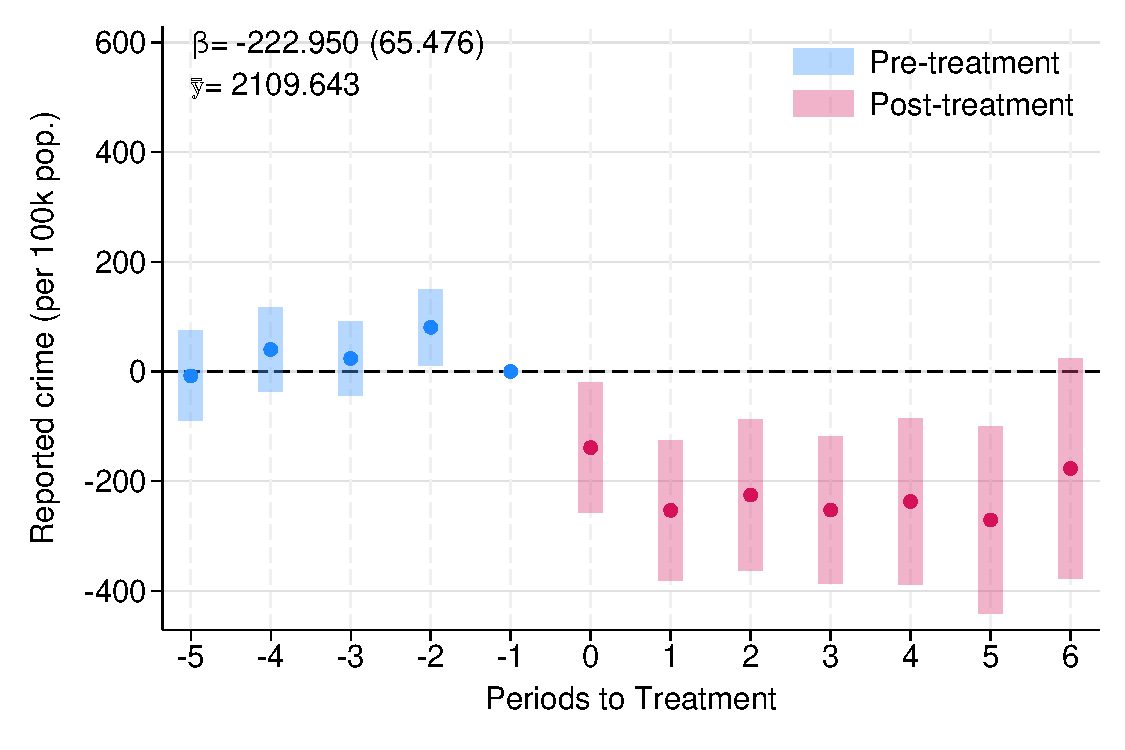
\includegraphics[width=\textwidth]{../manuscript/Graphs/DID2S_event_study_crime.pdf}
        \caption{Gardner}
    \end{subfigure}
    \\[6pt]
    \begin{subfigure}{0.47\textwidth}
        \centering
        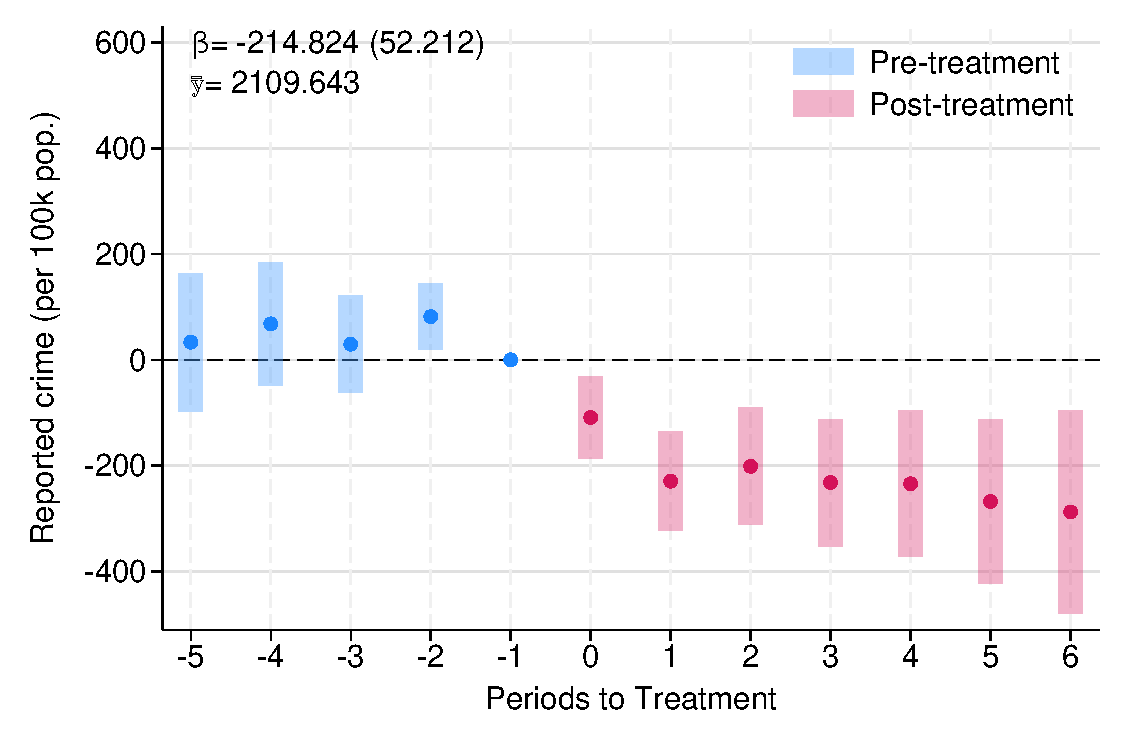
\includegraphics[width=\textwidth]{../manuscript/Graphs/JWDID_event_study_crime.pdf}
        \caption{Wooldridge}
    \end{subfigure}
    \\[12pt]
    \begin{minipage}{0.99\textwidth}
    \footnotesize Notes: The figure reports event-study estimates of the effect of \emph{Plan Cuadrante} on the number of crimes reported to the police in the municipality per 100,000 inhabitants using administrative data, estimated with three alternative difference-in-differences estimators robust to staggered adoption: \citet{Chaisemartin} in panel (a), \citet{Gardner} in panel (b), and \citet{wooldridge2023simple} in panel (c). Each panel plots the estimated coefficient at each event time relative to treatment along with 95\% confidence intervals. Standard errors are clustered at the municipality level. The headline coefficient $\beta$ is the equal-weighted average of the post-treatment effects from $t=0$ to $t=6$, and $\bar{y}$ denotes the never-treated mean of the outcome over the sample period.
    \end{minipage}
\end{figure}

\clearpage

\subsection{Effects of \emph{Plan Cuadrante} using a Balanced Panel}

Figure \ref{fig:figureA6_bp} shows the effects of \emph{Plan Cuadrante} on the main outcomes, but estimated using a balanced panel of municipalities. For the ENUSC-based outcomes, this panel includes only municipalities that implemented the \emph{Plan Cuadrante} between 2006 and 2009, which allows the construction of a balanced panel from t-2 to t+3 (31 municipalities). For the administrative outcomes, the balanced panel comprises those municipalities observed over that same t-2 to t+3 window around their own adoption (94 for reported crime and 78 for arrests). The resulting estimates are very similar to those presented in the main document.

\begin{figure}[h!]
    \centering
    \caption{Effects of \emph{Plan Cuadrante} Using a Balanced Panel of Municipalities}
    \label{fig:figureA6_bp}
    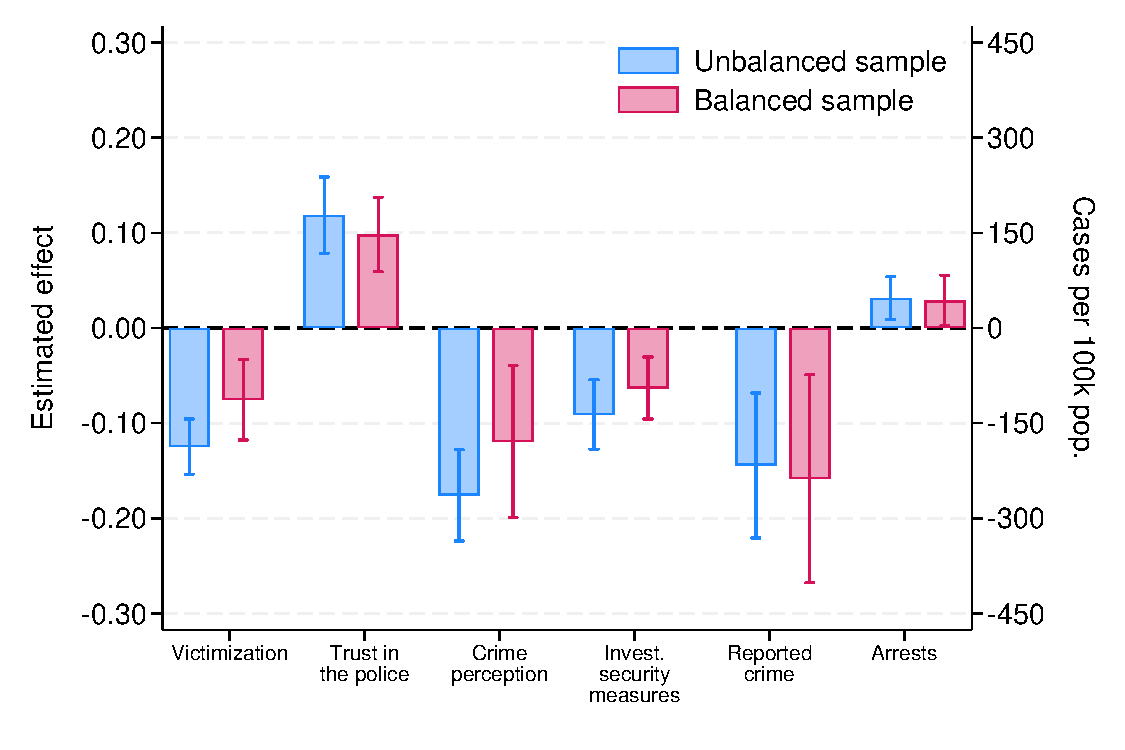
\includegraphics[width=0.8\textwidth]{../manuscript/Graphs/results_crime_balanced_combined.pdf}
    \\[10pt]
    \begin{minipage}{0.99\textwidth}
    \footnotesize Notes: The figure reports the effects of \emph{Plan Cuadrante} on different measures of police effectiveness using the main analytical sample (unbalanced, blue bars) and a balanced panel of municipalities observed over the full event-study window from $t-2$ to $t+3$ (red bars). For the ENUSC sample the balanced panel consists of the 31 municipalities that implemented \emph{Plan Cuadrante} between 2006 and 2009; for the administrative municipality-level sample it consists of 94 municipalities for reported crime and 78 municipalities for arrests. The bars represent the average post-treatment effect estimated with the difference-in-differences estimator developed in \citet{Callaway}, and the whiskers the 95\% confidence intervals; standard errors are clustered at the municipality level. Victimization is the probability of household victimization in the last 12 months; reported crime is the number of crimes reported to the police in the municipality per 100,000 inhabitants; arrests is the number of arrests per 100,000 inhabitants; trust in the police is the probability of reporting high trust in the police; crime perception is the probability of perceiving an increase in crime; and investment in security measures is the probability of adopting security measures in the last twelve months. Reported crime and arrests (administrative data) are read on the right axis; all other outcomes, from the ENUSC survey, are read on the left axis.
    \end{minipage}
\end{figure}

\clearpage

\subsection{Effects of \emph{Plan Cuadrante} Using the Full Set of Post-treatment and Pre-treatment Periods}
\label{sec:admin_uncapped}

For symmetry with the ENUSC-based analysis, the event studies for reported crime and arrests reported in the main text are restricted to 5 pre-treatment and 7 post-treatment periods. Because the administrative data are available for the full set of Chilean municipalities and therefore include a much larger number of never-treated municipalities than the ENUSC sample, we can estimate these effects over a longer window without exhausting the pool of valid comparison units. Figure \ref{fig:admin_uncapped} reports the effects of \emph{Plan Cuadrante} on reported crime and arrests using the full set of post-treatment and pre-treatment periods rather than capping the event study to the 5 pre-treatment and 7 post-treatment periods used in the main specification. The results are very similar to those presented in Section \ref{main_results}.

\begin{figure}[h!]
    \centering
    \caption{Effects of \emph{Plan Cuadrante} on Reported Crime and Arrests Using the Full Set of Post-treatment and Pre-treatment Periods}
    \label{fig:admin_uncapped}
    \begin{subfigure}{0.495\textwidth}
        \centering
        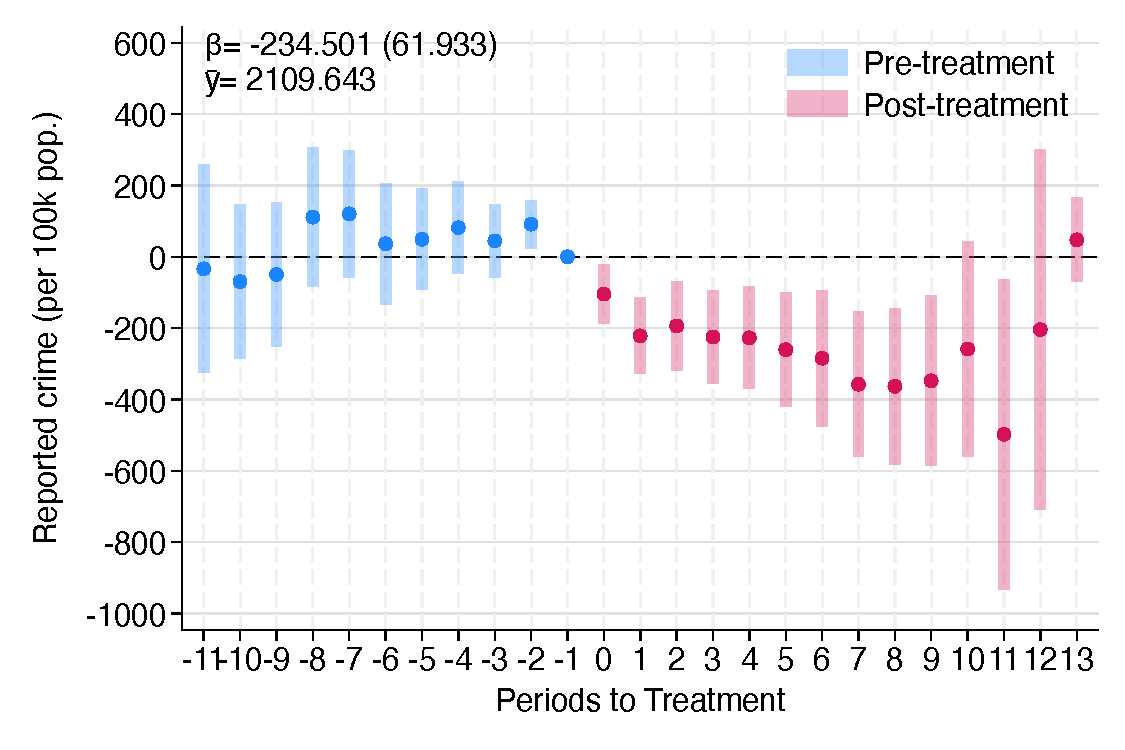
\includegraphics[width=0.98\textwidth]{../manuscript/Graphs/totalreportedcrime_allcomunas_uncapped.pdf}
        \caption{Reported crime per 100k inhabitants}
    \end{subfigure}%
    ~
    \begin{subfigure}{0.495\textwidth}
    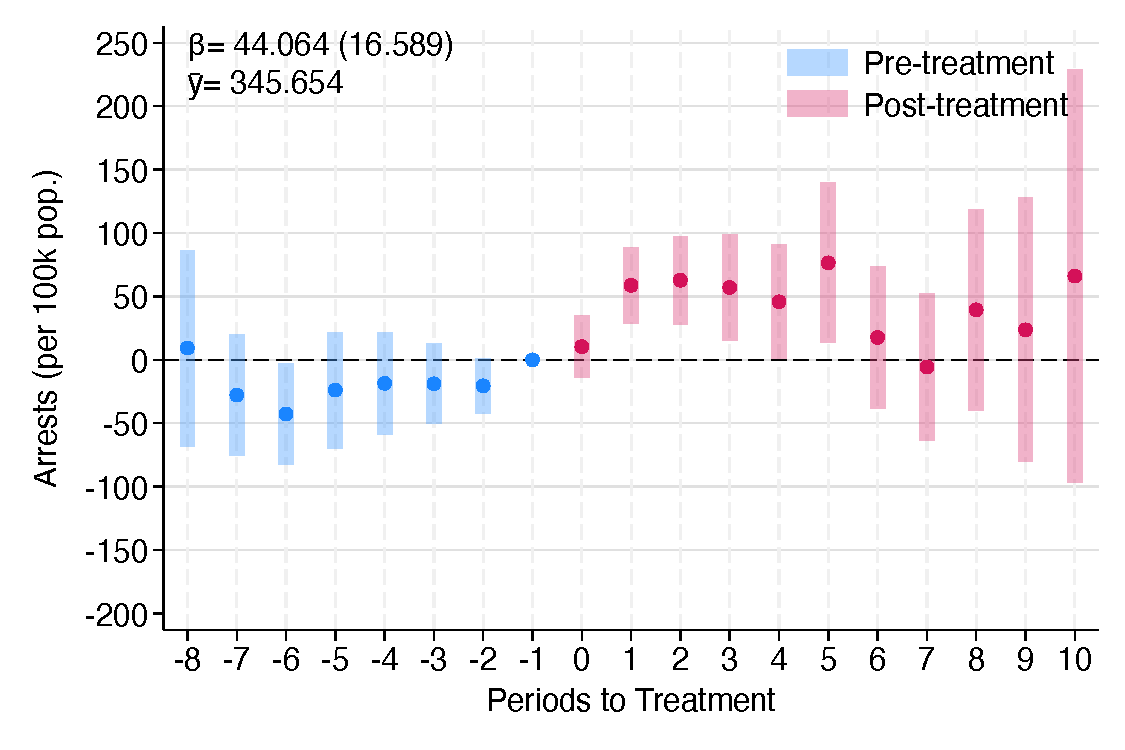
\includegraphics[width=0.98\textwidth]{../manuscript/Graphs/totalarrestscrime_allcomunas_uncapped.pdf}
        \caption{Arrests per 100k inhabitants}
    \end{subfigure}
    \begin{minipage}{\textwidth}
    \footnotesize
   Notes: This figure shows the dynamic effects of \emph{Plan Cuadrante} on the number of crimes reported to the police in the municipality per 100,000 inhabitants (panel a) and on the number of arrests in the municipality per 100,000 inhabitants (panel b), using administrative data. The estimation is conducted using the procedure developed in \citet{Callaway} for difference-in-differences with staggered treatment adoption. The dots in the figure represent the estimated coefficients and the bars behind them 95\% confidence intervals. Standard errors are clustered at the municipality level using the wild bootstrapping procedure. The pooled effect and the mean outcome before the introduction of the treatment are also presented in each panel. Unlike Figure \ref{fig:figure02} in the main text, we do not cap the event study to the same 5 pre-treatment and 6 post-treatment periods used for symmetry with the ENUSC-based analysis. Instead, we exploit the full set of post-treatment and pre-treatment periods. Panel (a) includes 4,371 observations and panel (b) 3,372 observations.
    \end{minipage}
\end{figure}

\clearpage

\subsection{Multiple Hypothesis Testing}
\label{sec:bonferroni}

Testing multiple outcomes simultaneously raises concerns about false discoveries. In our analyses, all six outcomes in our main analyses are statistically significant at the 1\% significance level. Under the null hypothesis of no effects, one would expect at most 1\% of tested coefficients to be false positives by chance at the same level. The observed pattern of results is therefore difficult to reconcile with false discoveries driven by multiple testing. Nonetheless, to address this concern formally, we apply a multiple hypothesis testing correction to the p-values. While procedures such as \citet{romano2005} would be a natural choice, their implementation is not computationally straightforward with the \citet{Callaway} estimator. We therefore apply the Bonferroni correction, which can be applied directly to any set of estimated p-values regardless of the underlying estimator. The adjusted p-values, reported in Table \ref{tab:bonferroni}, confirm that the main results remain statistically significant at conventional confidence levels after correction for every outcome considered.

\begin{table}[H]
\centering
\caption{Multiple Hypothesis Testing: Bonferroni Correction}
\label{tab:bonferroni}
\begin{tabular}{lcccc}
\toprule
Outcome & \multicolumn{2}{c}{} & \multicolumn{2}{c}{Bonferroni} \\
 & \multicolumn{2}{c}{Original} & \multicolumn{2}{c}{adjusted} \\
\cmidrule(lr){2-3} \cmidrule(lr){4-5}
 & p-value & & p-value & \\
\midrule
Victimization & 0.00000 & *** & 0.00000 & *** \\
Reported crime (per 100k pop.) & 0.00021 & *** & 0.00126 & *** \\
Crime perception & 0.00000 & *** & 0.00000 & *** \\
Investment in security measures & 0.00000 & *** & 0.00000 & *** \\
Trust in the police & 0.00000 & *** & 0.00000 & *** \\
Arrests (per 100k pop.) & 0.00316 & *** & 0.01896 & ** \\
\midrule
\multicolumn{5}{l}{\footnotesize Notes: Bonferroni correction multiplies each p-value by the number of} \\
\multicolumn{5}{l}{\footnotesize outcomes tested ($n=6$). Significance levels: *** $p<0.01$, ** $p<0.05$, * $p<0.1$.}
\end{tabular}
\end{table}
\clearpage

\subsection{Placebo Test Using Non-neighborhood Crime}

To assess whether the observed decline in crime is driven by broader temporal trends rather than increased police presence, we conduct a placebo test using a type of crime unlikely to be affected by beat policing—namely, non-neighborhood crime such as sexual abuse. These crimes typically occur outside the scope of routine neighborhood patrols and are therefore not expected to respond directly to changes in local police deployment. We use annual municipal-level data on reported sexual abuse and related arrests from 2005 to 2016, obtained from the Undersecretary for Crime Prevention.

Figure~\ref{fig:figureA9} shows that the implementation of \emph{Plan Cuadrante} is, as expected, not significantly associated with changes in sexual abuse crime.

\begin{figure}[h!]
    \centering
    \caption{The Effects of \emph{Plan Cuadrante} on Sexual Abuse}
    \label{fig:figureA9}
    \begin{subfigure}{0.495\textwidth}
        \centering
        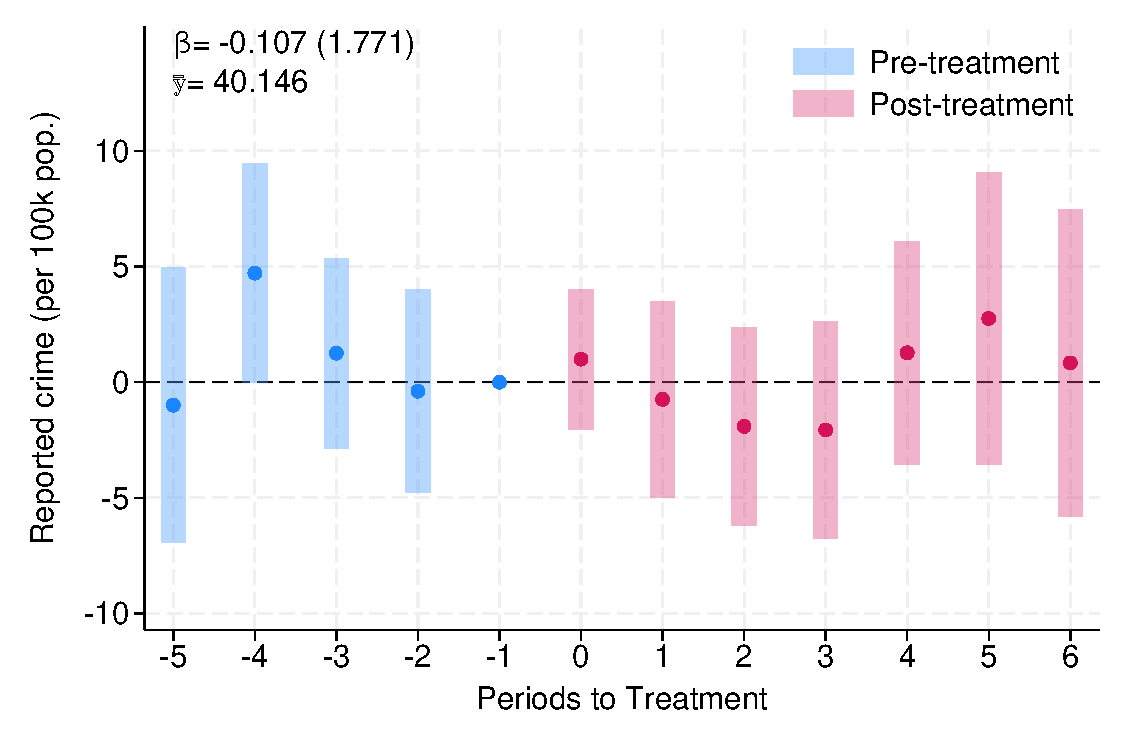
\includegraphics[width=\textwidth]{../manuscript/Graphs/results_sexualabuse.pdf}
                \caption{Reported crime per 100k inhabitants}
    \end{subfigure}%
    ~
    \begin{subfigure}{0.495\textwidth}
        \centering
        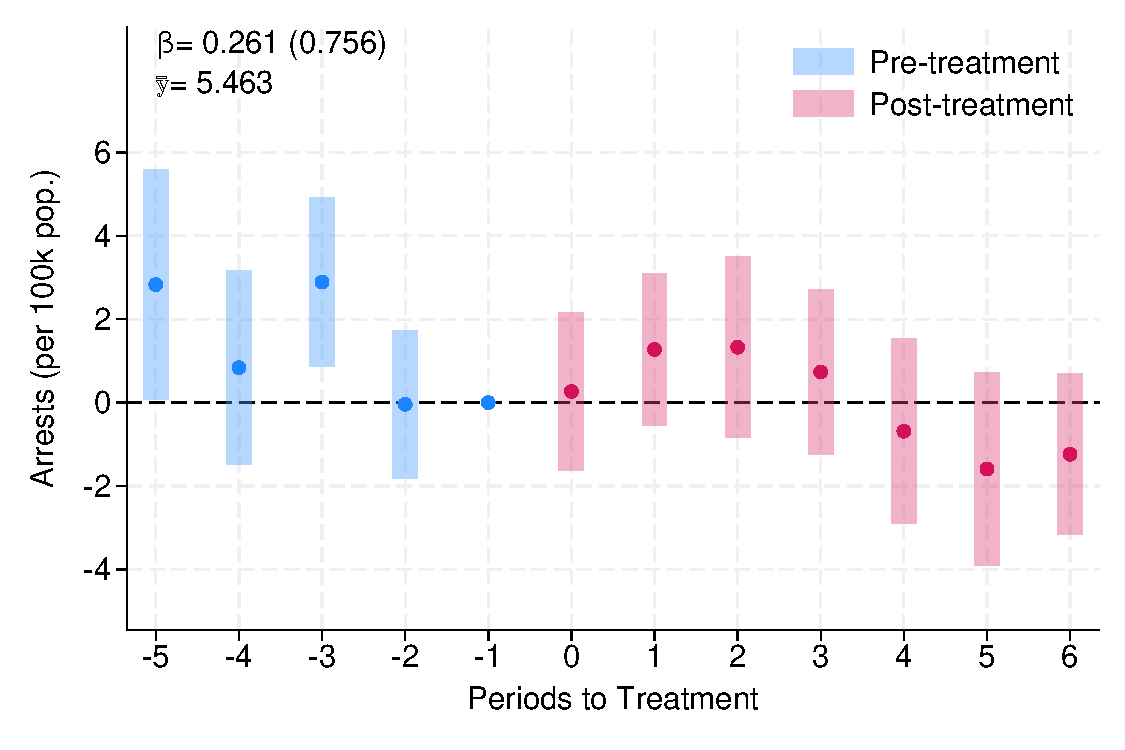
\includegraphics[width=\textwidth]{../manuscript/Graphs/results_sexualabuse2.pdf}
                \caption{Arrests per 100k inhabitants}
    \end{subfigure}
    \\[12pt]
    \begin{minipage}{0.99\textwidth}
    \footnotesize Notes: This figure shows the dynamic effects of the \emph{Plan Cuadrante} on sexual abuse per 100,000 inhabitants. The estimation is conducted using the procedure developed in \citet{Callaway} for difference-in-differences with staggered treatment adoption. The graphs display the estimated coefficients and 95\% confidence intervals. Standard errors are clustered at the municipality level using the wild bootstrapping procedure.
    \end{minipage}
\end{figure}
\clearpage

\subsection{The Effects of \emph{Plan Cuadrante} on Other Measures of Crime Perception}

The results reported in panel (c) of Figure \ref{fig:figure02} showed that \emph{Plan Cuadrante} decreased households' perception of crime in the neighborhood. However, the ENUSC survey not only asks about individuals' crime perception in the neighborhood, but also in the municipality and in the country. Figure \ref{fig:figureA3} reports the results of \emph{Plan Cuadrante} on the perception of crime in the municipality and in the country. While the effect is consistently negative and statistically significant also for these measures of crime perception, the effect is much smaller for insecurity in the country, indicating that the effects of the program on crime perception are larger at the local level.

\begin{figure}[h!]
    \centering
    \caption{Effects of \emph{Plan Cuadrante} on Crime Perception in the Municipality and in the Country}
    \label{fig:figureA3}
    \begin{subfigure}{0.495\textwidth}
        \centering
        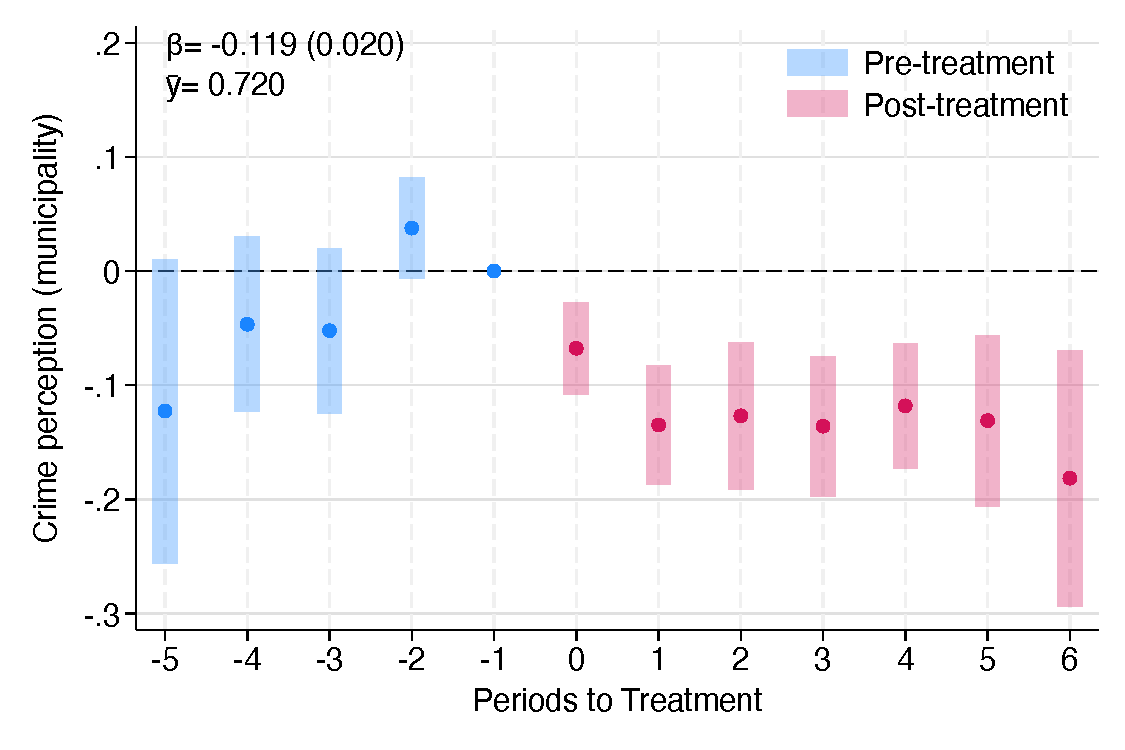
\includegraphics[width=\textwidth]{../manuscript/Graphs/results_perception_municipality.pdf}
        \caption{In the municipality}
    \end{subfigure}%
    ~ 
    \begin{subfigure}{0.495\textwidth}
    \centering
    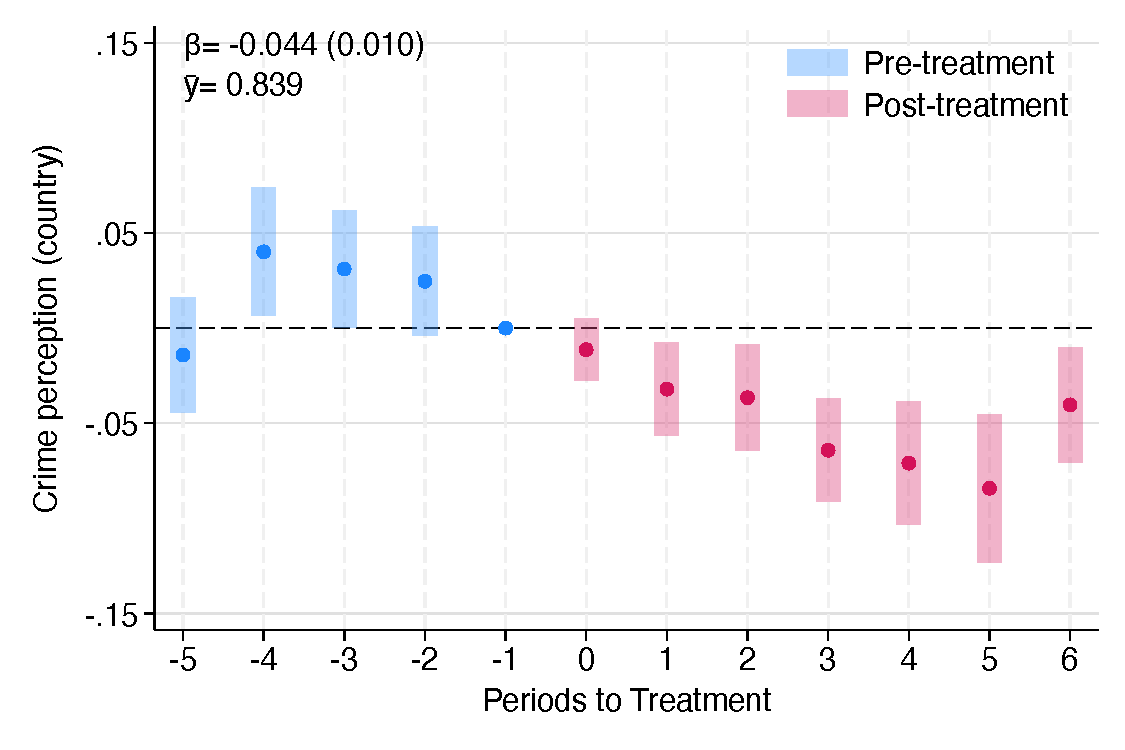
\includegraphics[width=\textwidth]{../manuscript/Graphs/results_perception_country.pdf}
        \caption{In the country}
    \end{subfigure}
    \\[12pt]
    \begin{minipage}{0.99\textwidth}
    \footnotesize Notes: This figure shows the dynamic effects of the \emph{Plan Cuadrante} on the proportion of individuals that perceive an increase in crime in the municipality in the last 12 months (panel a), and on the proportion of individuals that perceive an increase in crime in the country in the last 12 months (panel b). Panel (a) includes 90,696 observations, while panel (b) includes 92,305 observations. The estimation is conducted using the procedure developed in \citet{Callaway} for difference-in-differences with staggered treatment adoption. The dots in the figure represent the estimated coefficients and the bars behind them 95\% confidence intervals. Standard errors are clustered at the municipality level using the wild bootstrapping procedure. The pooled effect and the mean outcome before the introduction of the treatment for every outcome---computed as in Figure \ref{fig:figure02}, using only the pre-treatment observations of treated units---is also presented in each panel.
    \end{minipage}
\end{figure}



 
\clearpage

\subsection{Robustness to the 2010 Earthquake}
\label{sec:earthquake}

The 2010 Maule earthquake could confound our estimates if it differentially affected treated and control municipalities, either by disrupting police operations and thus reducing treatment intensity, or by independently affecting crime perceptions and security outcomes in ways unrelated to \emph{Plan Cuadrante}. To address this concern, we re-estimate our main results excluding municipalities more exposed to the earthquake, defined as those experiencing a Modified Mercalli Intensity greater than 7. This corresponds to 21 municipalities in the ENUSC sample and 158 municipalities in the administrative data sample. The results, reported in Figure \ref{fig:figure02_noEQ}, are nearly identical to the main estimates, confirming that the 2010 earthquake does not drive our findings.

%--- Robustness check: 2010 Maule earthquake (Mercalli > 7 excluded)
\begin{figure}[h!]
    \centering
    \caption{Effects of \emph{Plan Cuadrante} excluding Municipalities Affected by the 2010 Earthquake}
    \label{fig:figure02_noEQ}
    \begin{subfigure}{0.495\textwidth}
        \centering
        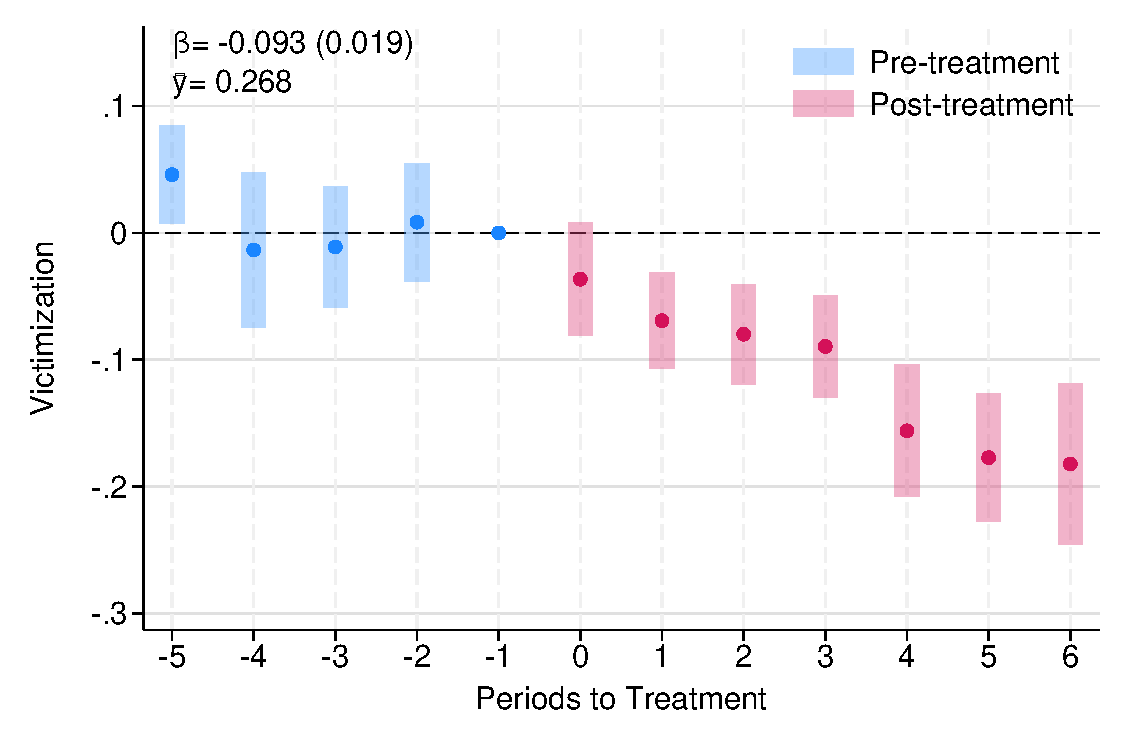
\includegraphics[width=\textwidth]{../manuscript/Graphs/results_victimization_noEQ.pdf}
        \caption{Victimization in last 12 months}
    \end{subfigure}%
    ~
    \begin{subfigure}{0.495\textwidth}
        \centering
        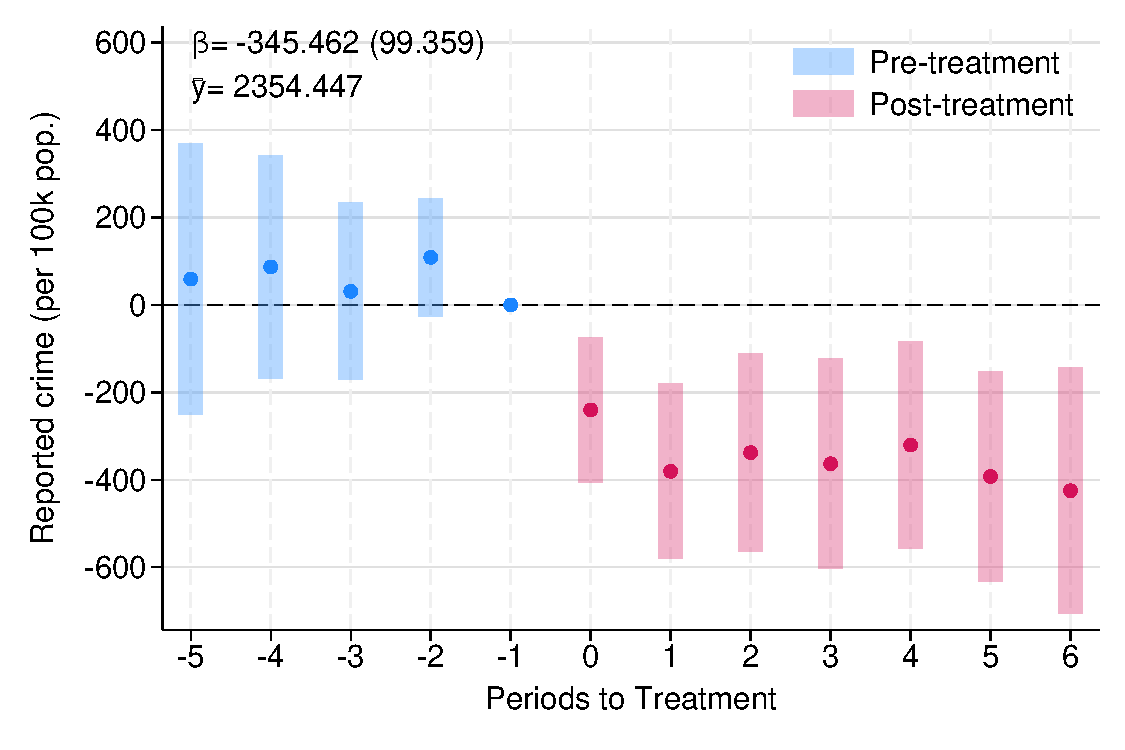
\includegraphics[width=\textwidth]{../manuscript/Graphs/totalreportedcrime_allcomunas_noEQ.pdf}
        \caption{Reported crime per 100k inhabitants}
    \end{subfigure}
    \begin{subfigure}{0.495\textwidth}
        \centering
        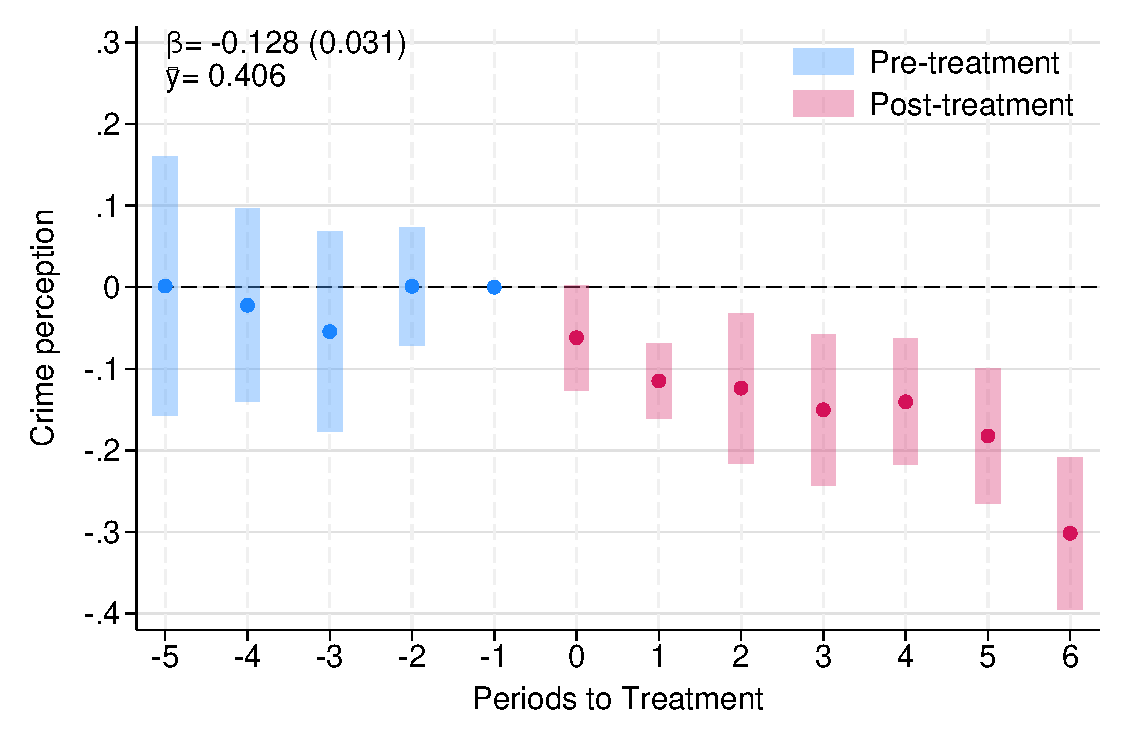
\includegraphics[width=\textwidth]{../manuscript/Graphs/results_perception_noEQ.pdf}
        \caption{Households reporting an increase in crime}
    \end{subfigure}%
    ~
    \begin{subfigure}{0.495\textwidth}
        \centering
        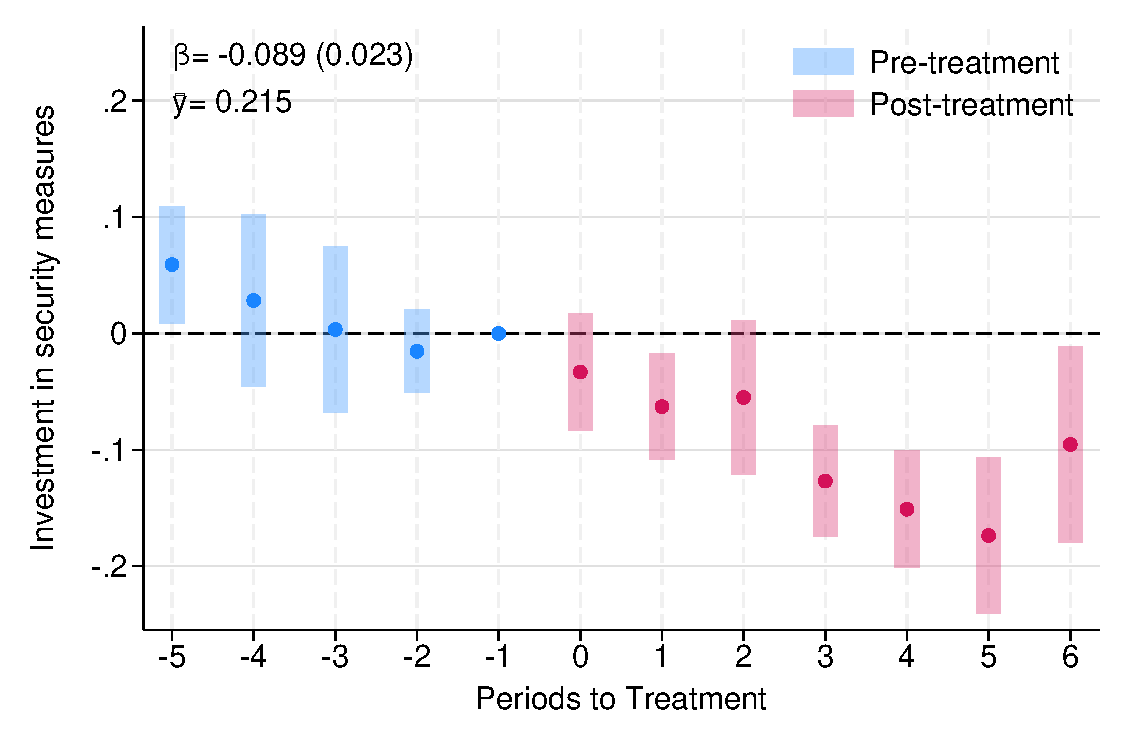
\includegraphics[width=\textwidth]{../manuscript/Graphs/results_hhprotectionmeasures_noEQ.pdf}
        \caption{Households adopting security measures}
    \end{subfigure}
    \\[12pt]
    \begin{minipage}{0.99\textwidth}
    \footnotesize
    Notes: This figure replicates the results of Figure \ref{fig:figure02} after excluding municipalities affected by the 2010 Maule earthquake, defined as those with a Modified Mercalli Intensity (MMI) score strictly greater than 7. The estimation is conducted using the procedure developed in \citet{Callaway} for difference-in-differences with staggered treatment adoption. The dots in the figure represent the estimated coefficients and the bars behind them 95\% confidence intervals. Standard errors are clustered at the municipality level using the wild bootstrapping procedure. The pooled effect and the mean outcome before the introduction of the treatment is also presented in each panel. Panel (a) reports the effect of \emph{Plan Cuadrante} on the probability of household victimization in the last 12 months using the ENUSC survey. Panel (b) reports the effect on the number of crimes reported to the police in the municipality per 100,000 inhabitants using administrative data. Panel (c) reports the effect on the probability of perceiving an increase in crime using the ENUSC survey. Panel (d) reports the effect on the probability of adopting security measures in the last twelve months using the ENUSC survey.
    \end{minipage}
\end{figure}

\clearpage

\subsection{Randomization-Inference Placebo Test}
\label{sec:ri_appendix}

As a further robustness check, we implement a placebo/randomization-inference exercise: we reassign adoption dates and never-treated status at random and re-estimate our specification under the sharp null of no treatment effect for any unit. The estimated direct effect on treated municipalities falls in the bottom first percentile of the resulting placebo distribution, while the analogous estimate for untreated neighbors of treated municipalities falls near its center---between the 40th and 45th percentile---consistent with a genuine effect on treated municipalities and with the absence of spillovers documented in Online Appendix \ref{spillovers} below.

For this exercise, we reassign adoption dates and never-treated status across municipalities $1{,}000$ times and re-estimate the direct and spillover effects under the sharp null, yielding the placebo distributions in Online Appendix Figure~\ref{fig:ri_placebo}. We rely on the estimator of \citet{Chaisemartin} rather than that of \citet{Callaway} for this exercise: re-estimating the latter over a thousand permutations would require prohibitive computational power and running time.

\begin{figure}[h!]
    \centering
    \caption{Randomization Inference for the Direct and Spillover Effects of \emph{Plan Cuadrante}}
    \label{fig:ri_placebo}
    \begin{subfigure}{0.495\textwidth}
        \centering
        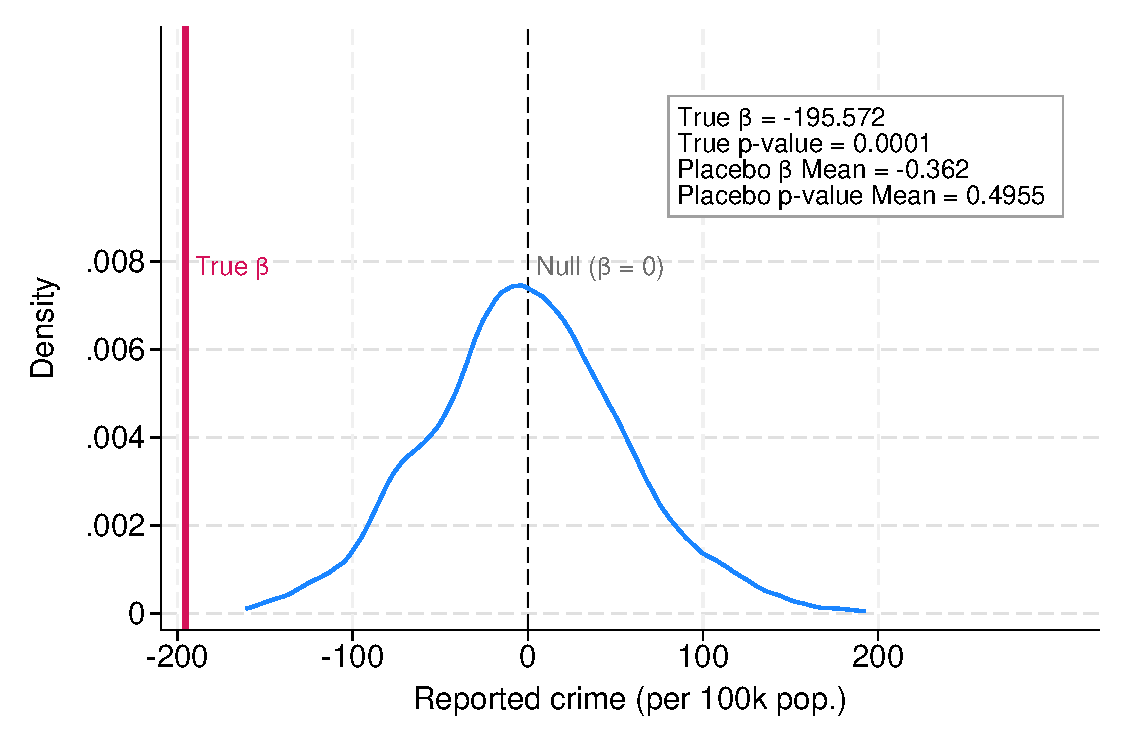
\includegraphics[width=\textwidth]{../manuscript/Graphs/CHDH_RI_placebo_crime.pdf}
        \caption{Reported crime}
        \label{fig:ri_crime}
    \end{subfigure}%
    ~
    \begin{subfigure}{0.495\textwidth}
        \centering
        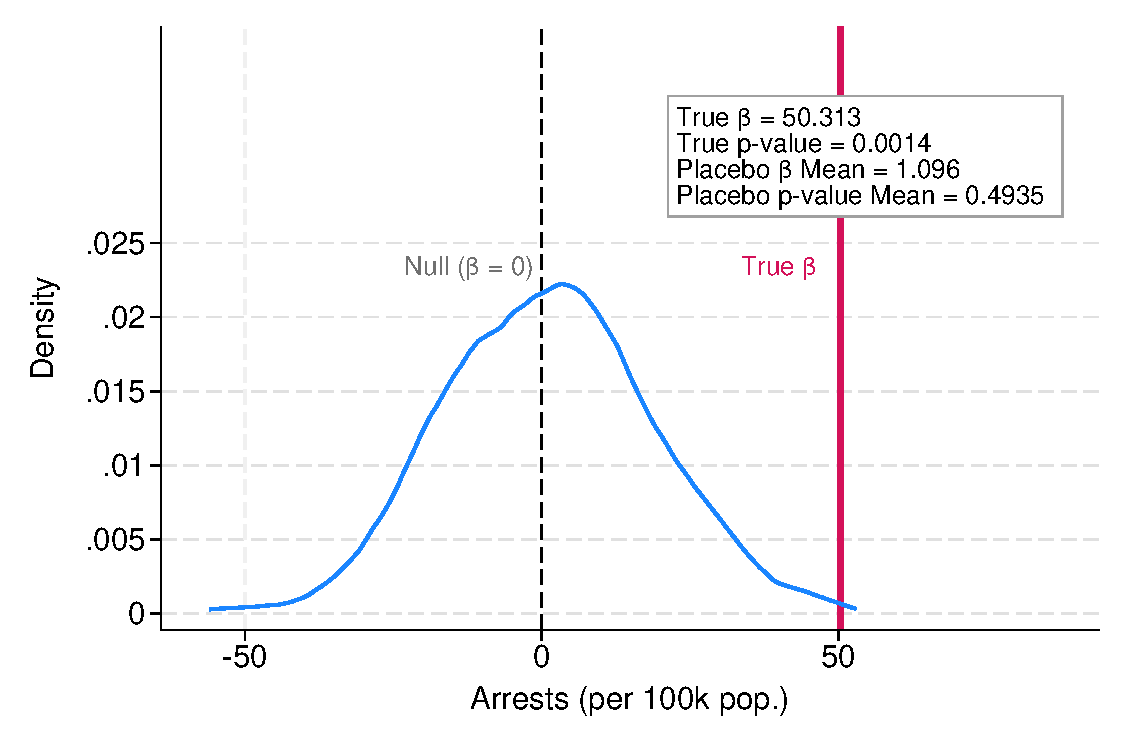
\includegraphics[width=\textwidth]{../manuscript/Graphs/CHDH_RI_placebo_arrests.pdf}
        \caption{Arrests}
        \label{fig:ri_arrests}
    \end{subfigure}

    \begin{subfigure}{0.495\textwidth}
        \centering
        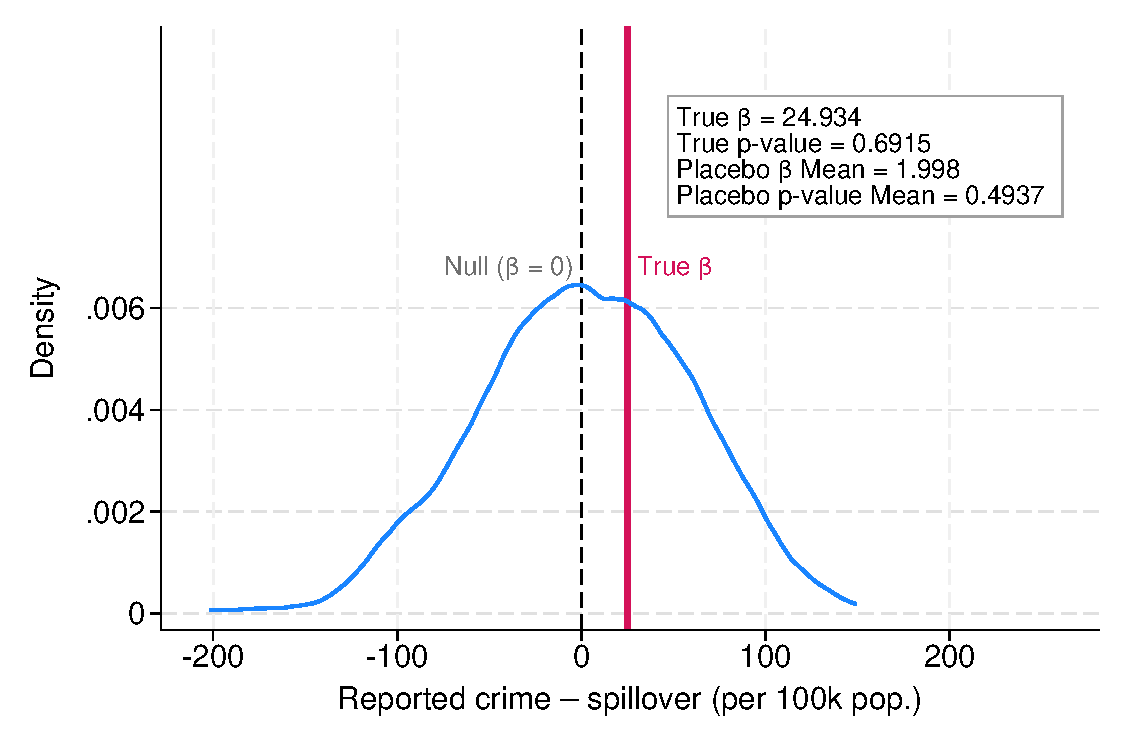
\includegraphics[width=\textwidth]{../manuscript/Graphs/CHDH_RI_placebo_crime_spillover.pdf}
        \caption{Spillovers on Reported crime}
        \label{fig:ri_crime_spillover}
    \end{subfigure}%
    \begin{subfigure}{0.495\textwidth}
        \centering
        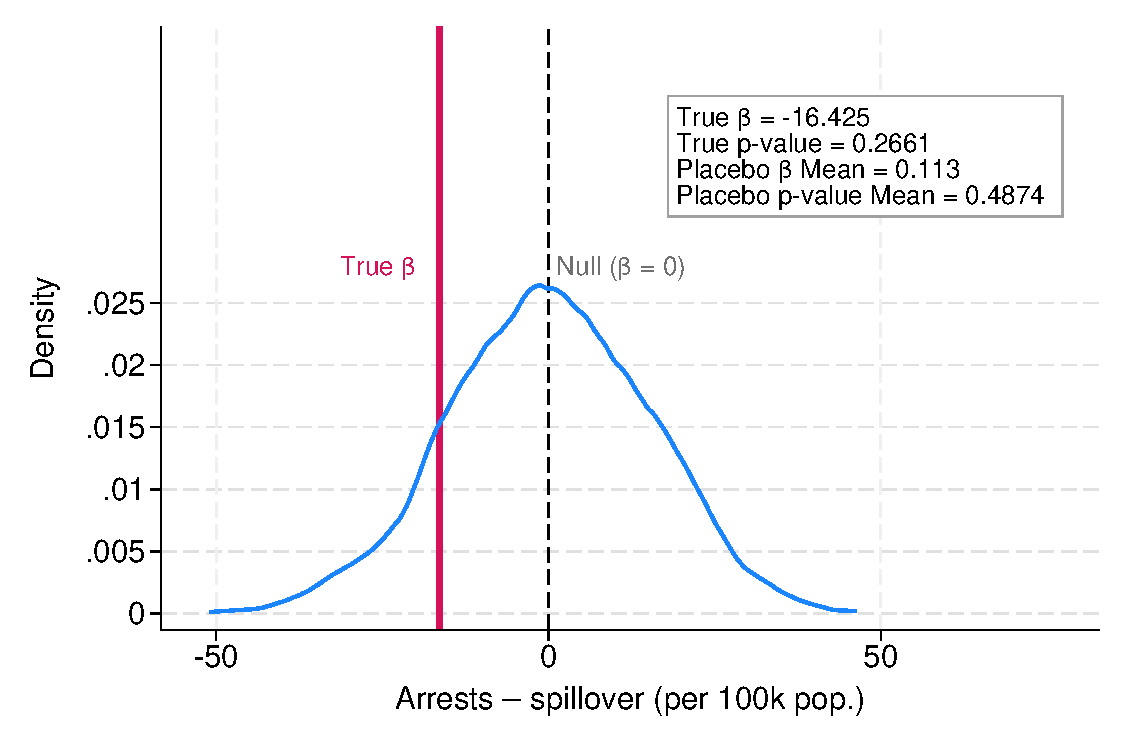
\includegraphics[width=\textwidth]{../manuscript/Graphs/CHDH_RI_placebo_arrests_spillover.pdf}
        \caption{Spillovers on Arrests}
        \label{fig:ri_arrests_spillover}
    \end{subfigure}
    \begin{minipage}{0.95\textwidth}
    \footnotesize
    Notes: This figure presents randomization inference results under the sharp null of no treatment effect, using the heterogeneity-robust estimator of \citet{Chaisemartin}. Each curve is the kernel density of 1{,}000 placebo ATT estimates obtained by jointly permuting \emph{Plan Cuadrante} adoption dates and never-treated status across municipalities (drawing from the empirical distribution of (date, status) pairs, so the marginal counts of treated and never-treated municipalities are preserved in every permutation). In each permutation the variable PC is shuffled across all 346 municipalities and a new time-varying treatment indicator is computed before re-estimating the dynamic effects. The solid colored vertical line marks the point estimate from the true rollout; the dashed black line marks the null expectation $\beta = 0$. The boxes report the true point estimate, its asymptotic two-sided $p$-value, and the mean of the placebo $\beta$ and placebo $p$-value distributions.
    \end{minipage}
\end{figure}

\clearpage

\subsection{Testing for Spatial Spillovers}
\label{spillovers}

This Online Appendix details the specifications behind the spillover tests summarized in Section~\ref{sec:spillovers}.

For the intensity-based test in the spirit of \citet{crepon2013}, we replace the binary neighbor-treatment indicator with a continuous measure of exposure and restrict the sample to never-treated municipalities,
\begin{equation}
Outcome_{mt}= \delta_{1}\,\mbox{\textit{Share neighbors with Plan Cuadrante}}_{mt} + Municipality_{m} + Year_{t} + u_{mt}
\label{eq:crepon}
\end{equation}
\noindent Because the treatment is continuous, we estimate it with the heterogeneity-robust estimator of \citet{Chaisemartin}, measuring exposure both as the share of treated neighbors (Online Appendix Figure~\ref{fig:figure_continuous_spillovers}) and as their number (Online Appendix Figure~\ref{fig:figure_count_spillovers}).

The baseline test estimates the effect of \emph{Plan Cuadrante} on reported crime, arrests, police officers, and patrol vehicles in neighboring untreated municipalities,
\begin{equation}
Outcome_{mt}= \delta_{1}\,\mbox{\textit{Plan Cuadrante near municip.}}_{mt} + Municipality_{m} + Year_{t} + u_{mt}
\label{eq:main3}
\end{equation}
\noindent where the sample is restricted to municipalities that never adopted the program, each is assigned a treatment date equal to the earliest adoption among its treated neighbors, and $\delta_{1}$ is estimated dynamically with the staggered difference-in-differences estimator of \citet{Callaway}. Because these administrative outcomes are observed for every municipality, we estimate the specification on the full national sample (Online Appendix Figure~\ref{fig:spillover_admin}).

Finally, we re-estimate the baseline administrative specification on the municipalities neighboring the 46 ENUSC municipalities (Online Appendix Figure~\ref{fig:figure_46ENUSC_spillovers_admin}); and, for the outcomes measured only in ENUSC, we estimate the spillover of early-adopting ENUSC municipalities on their late-adopting ENUSC neighbors before the latter's own adoption (Online Appendix Figure~\ref{fig:figure_results_spillovers_enusc}). The six focal late-adopters, each shown with its earliest-adopting ENUSC neighbor and that neighbor's adoption year, are Molina (Curic\'o, 2005), Tocopilla (Iquique, 2005), San Carlos (Chill\'an, 2007), Padre Hurtado (Pe\~naflor, 2008), Calera (Quillota, 2008), and Limache (Quillota, 2008). Across all of these specifications, the estimated spillover effects are small and statistically indistinguishable from zero.

\begin{figure}[h!]
    \centering
    \caption{Geographic Spillovers of \emph{Plan Cuadrante} by Share of Treated Neighbors}
    \label{fig:figure_continuous_spillovers}
    \begin{subfigure}{0.495\textwidth}
        \centering
        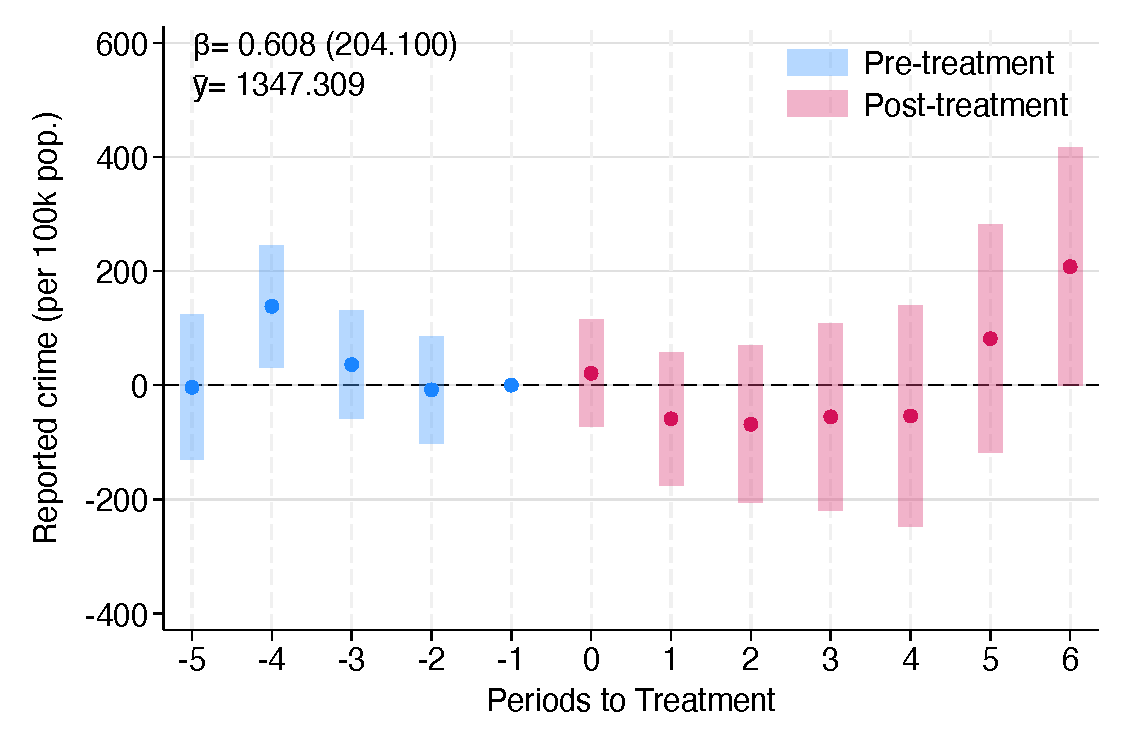
\includegraphics[width=0.98\textwidth]{../manuscript/Graphs/CHDH_continuous_spillover_crime.pdf}
        \caption{Spillovers on Reported Crime}
    \end{subfigure}%
    ~
    \begin{subfigure}{0.495\textwidth}
        \centering
        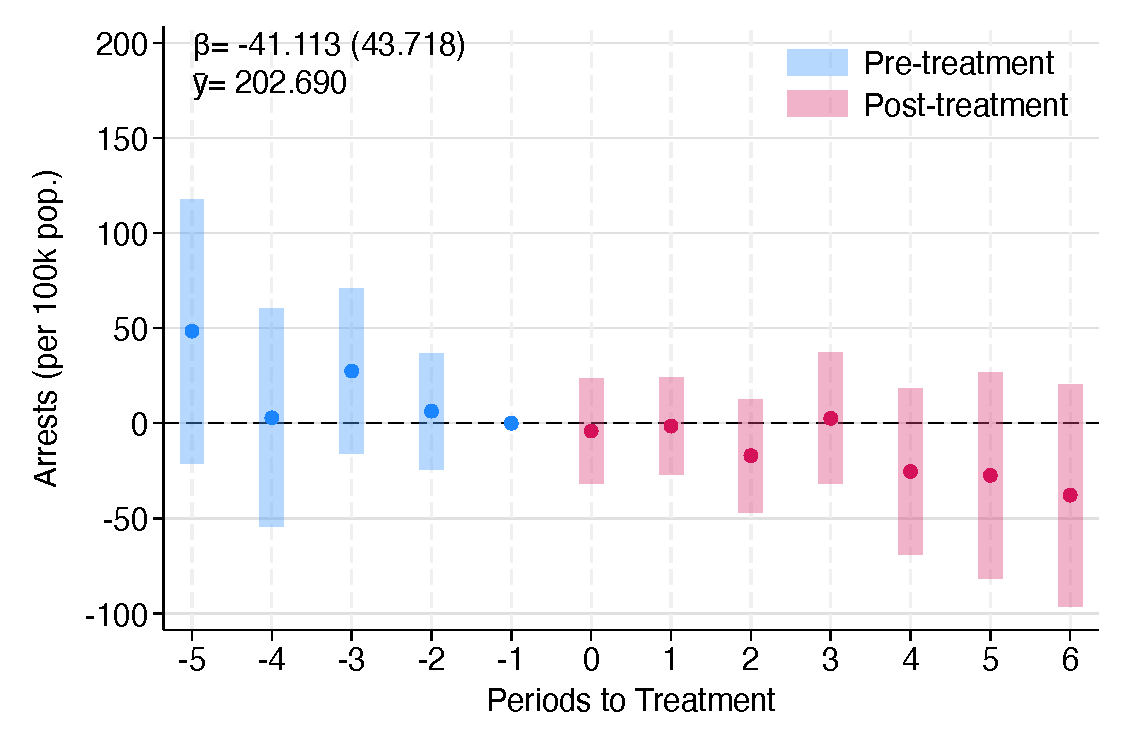
\includegraphics[width=0.98\textwidth]{../manuscript/Graphs/CHDH_continuous_spillover_arrests.pdf}
        \caption{Spillovers on Arrests}
    \end{subfigure}

    \vspace{0.5em}

    \begin{subfigure}{0.495\textwidth}
        \centering
        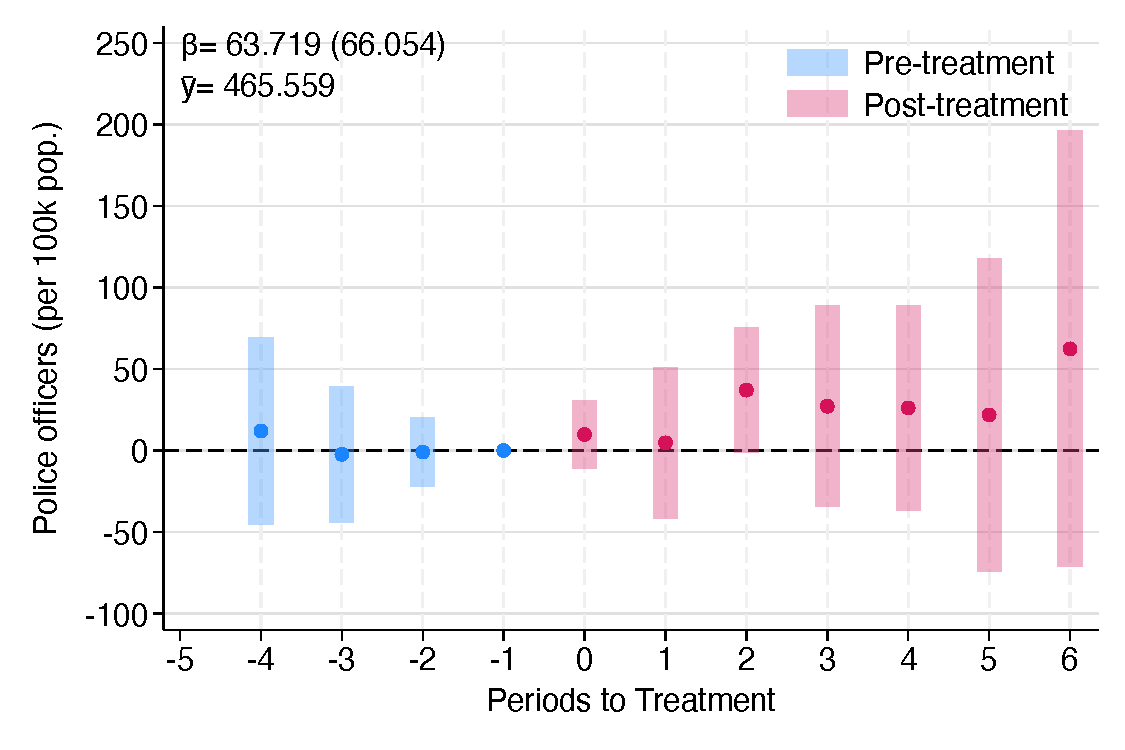
\includegraphics[width=0.98\textwidth]{../manuscript/Graphs/CHDH_continuous_spillover_dotpc.pdf}
        \caption{Spillovers on Police Officers}
    \end{subfigure}%
    ~
    \begin{subfigure}{0.495\textwidth}
        \centering
        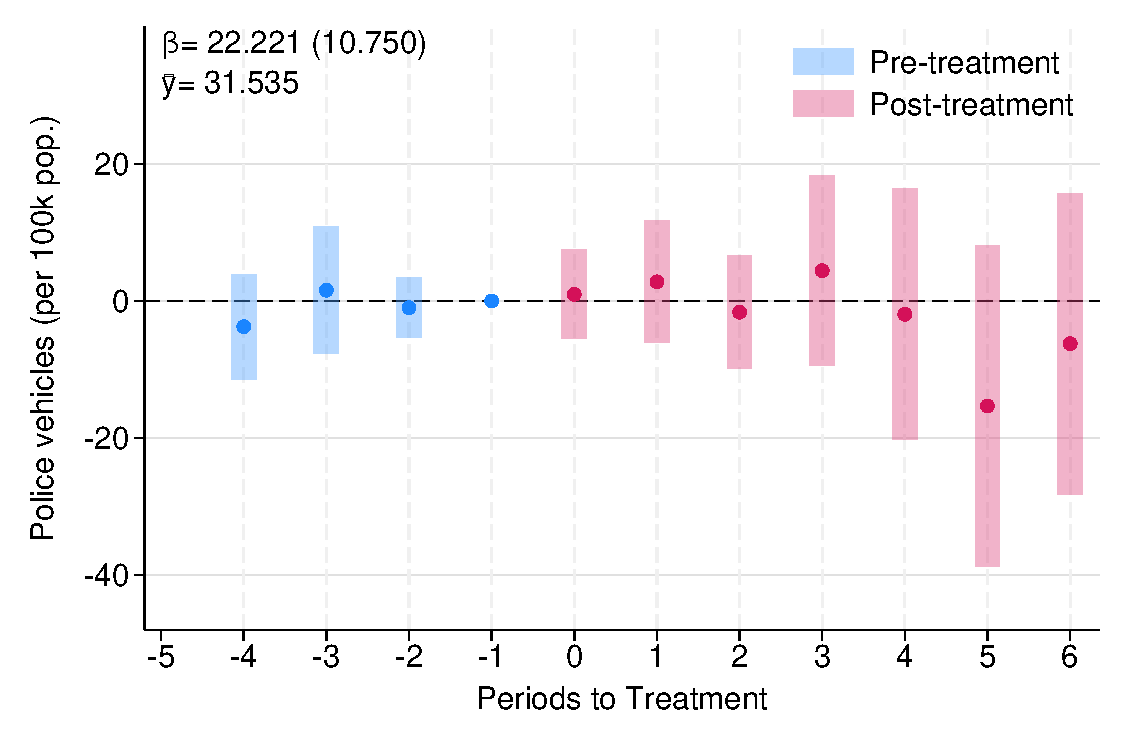
\includegraphics[width=0.98\textwidth]{../manuscript/Graphs/CHDH_continuous_spillover_vehiclespc.pdf}
        \caption{Spillovers on Patrol Vehicles}
    \end{subfigure}

    \begin{minipage}{0.95\textwidth}
    \footnotesize
    Notes: This figure reports the geographic spillover effects of \emph{Plan Cuadrante} on four outcomes for never-treated municipalities: reported crime per 100,000 inhabitants (panel a), arrests per 100,000 inhabitants (panel b), the number of police officers per 100,000 inhabitants (panel c), and the number of patrol vehicles per 100,000 inhabitants (panel d). Unlike the dummy spillover specification, the treatment variable is now continuous and equals the share of neighboring municipalities that have implemented \emph{Plan Cuadrante} by year $t$, following the spillover-intensity approach of \citet{crepon2013}. The sample is restricted to municipalities that never adopted \emph{Plan Cuadrante}. Estimation is performed using the heterogeneity-robust estimator of \citet{Chaisemartin}, which accommodates a continuous, time-varying treatment intensity in a staggered design. The dots represent the estimated dynamic effects and the bars behind them denote 95\% confidence intervals. Standard errors are clustered at the municipality level. The pooled effect  and the mean of the outcome among municipalities with no treated neighbors are reported in each panel.
    \end{minipage}
\end{figure}


\begin{figure}[h!]
    \centering
    \caption{Geographic Spillovers of \emph{Plan Cuadrante} by Number of Treated Neighbors}
    \label{fig:figure_count_spillovers}
    \begin{subfigure}{0.495\textwidth}
        \centering
        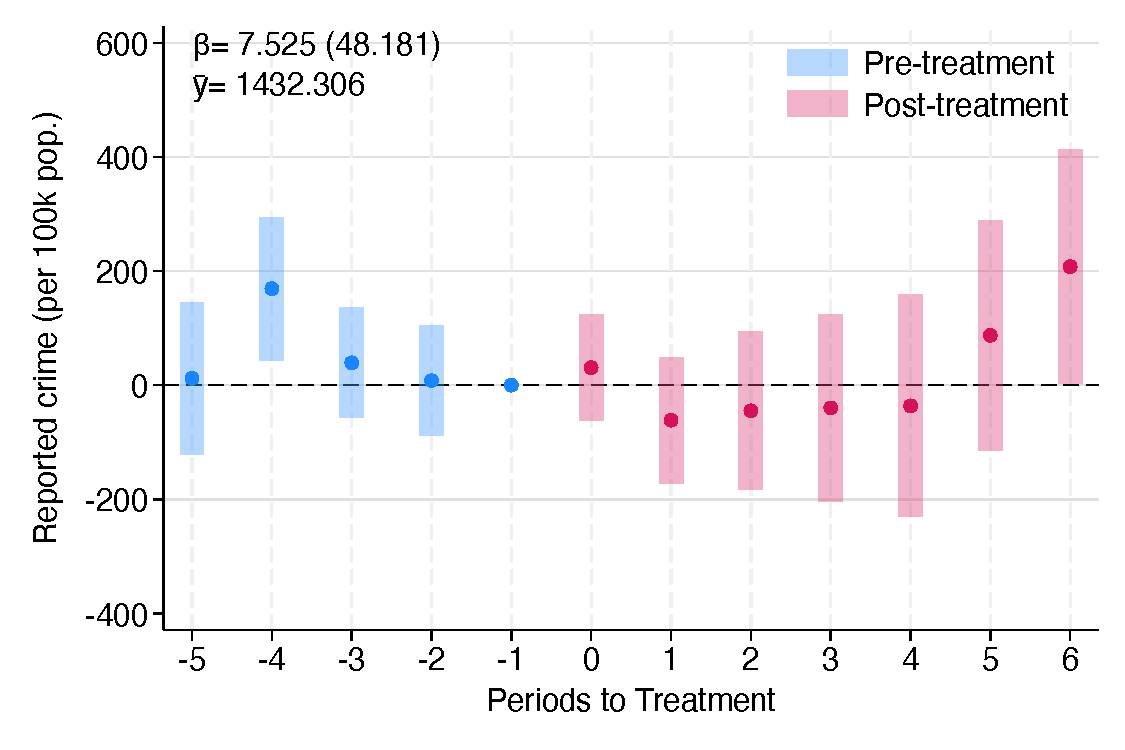
\includegraphics[width=0.98\textwidth]{../manuscript/Graphs/CHDH_continuous_spillover_crime_count.pdf}
        \caption{Spillovers on Reported Crime}
    \end{subfigure}%
    ~
    \begin{subfigure}{0.495\textwidth}
        \centering
        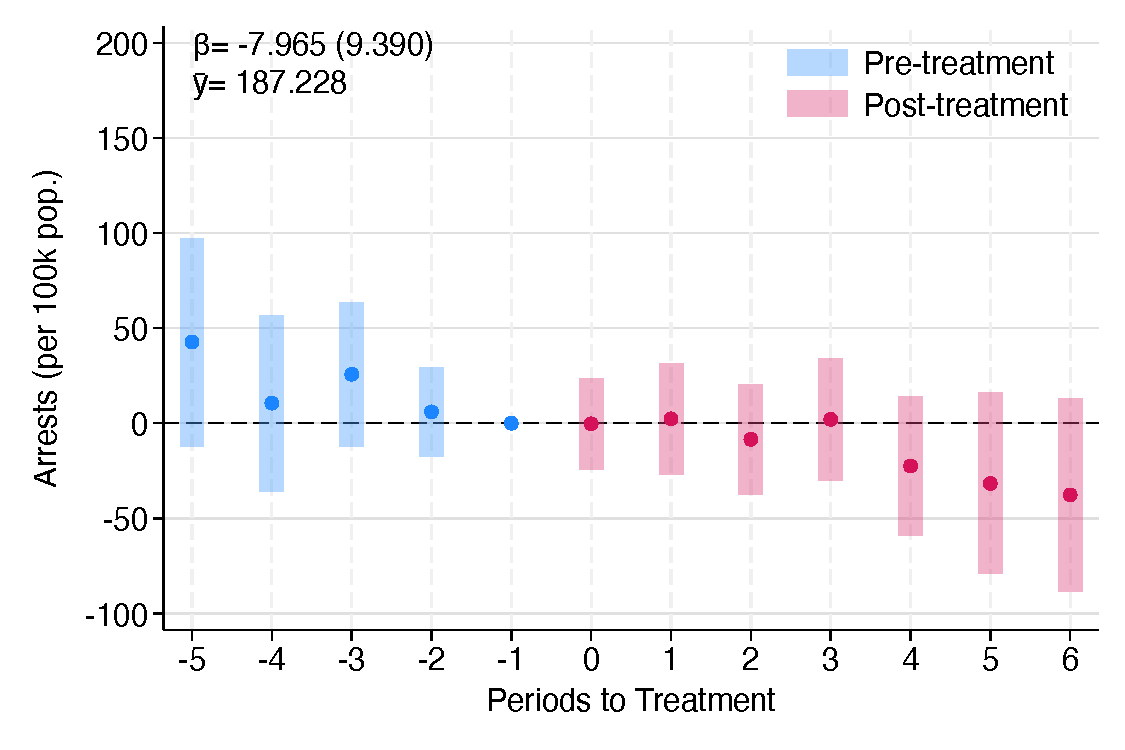
\includegraphics[width=0.98\textwidth]{../manuscript/Graphs/CHDH_continuous_spillover_arrests_count.pdf}
        \caption{Spillovers on Arrests}
    \end{subfigure}

    \vspace{0.5em}

    \begin{subfigure}{0.495\textwidth}
        \centering
        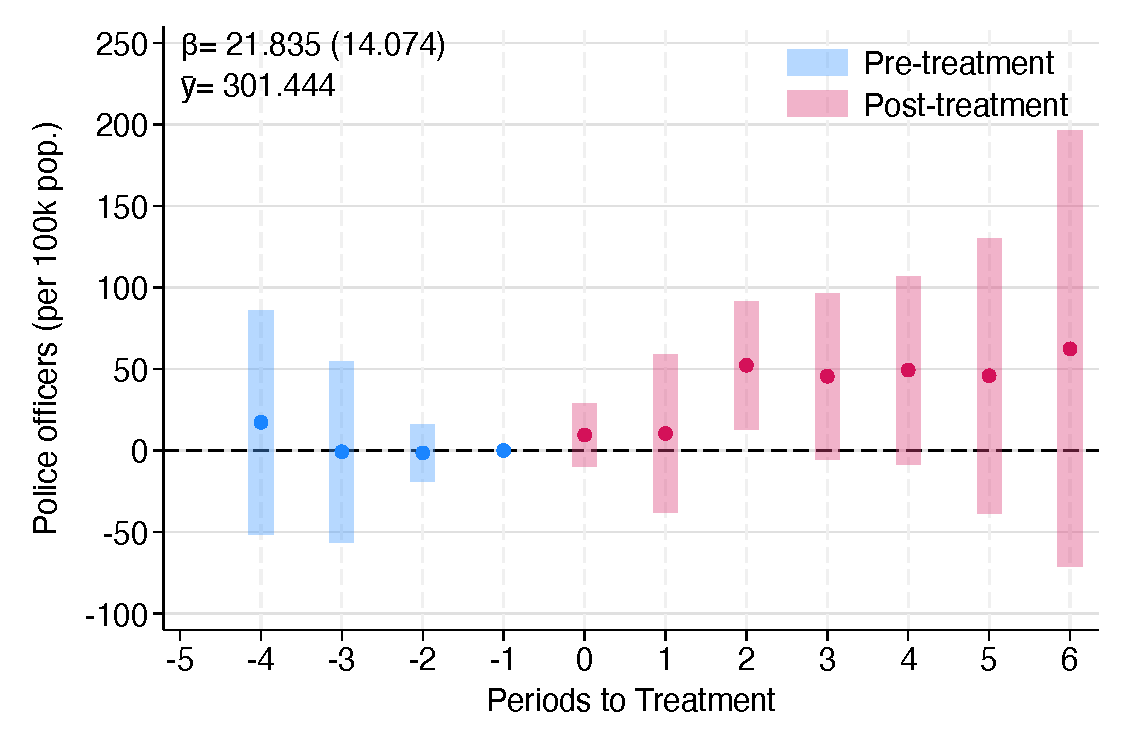
\includegraphics[width=0.98\textwidth]{../manuscript/Graphs/CHDH_continuous_spillover_dotpc_count.pdf}
        \caption{Spillovers on Police Officers}
    \end{subfigure}%
    ~
    \begin{subfigure}{0.495\textwidth}
        \centering
        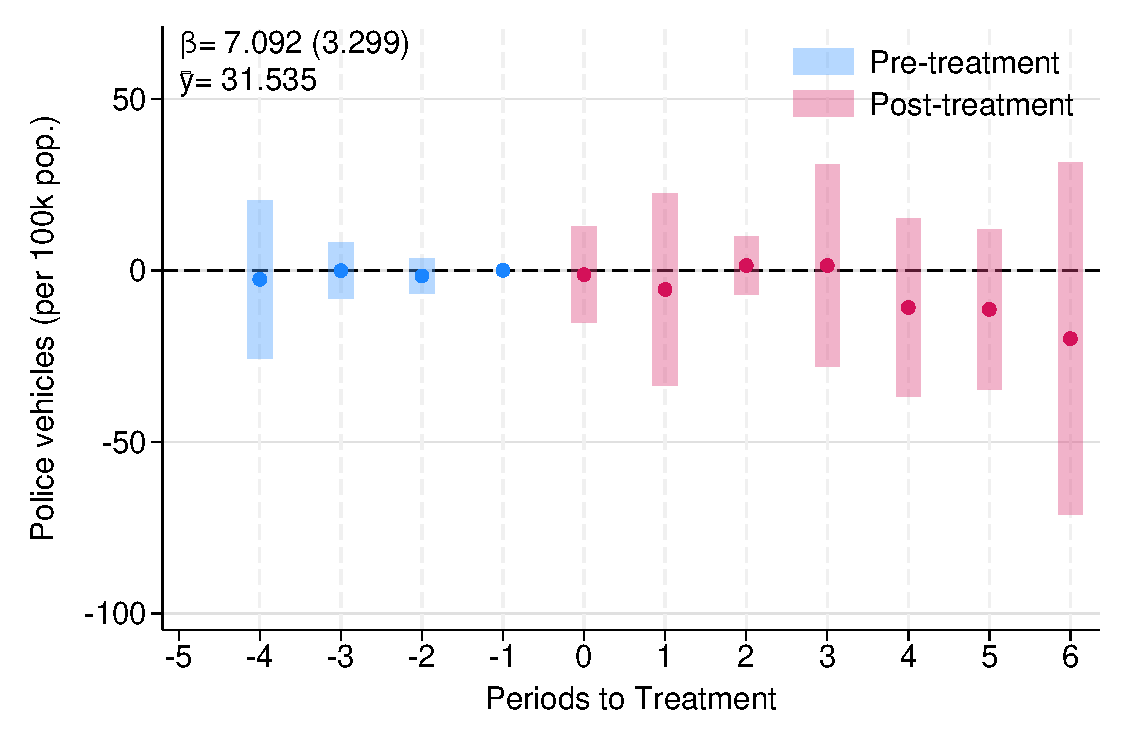
\includegraphics[width=0.98\textwidth]{../manuscript/Graphs/CHDH_continuous_spillover_vehiclespc_count.pdf}
        \caption{Spillovers on Patrol Vehicles}
    \end{subfigure}

    \begin{minipage}{0.95\textwidth}
    \footnotesize
    Notes: This figure reports the geographic spillover effects of \emph{Plan Cuadrante} on four outcomes for never-treated municipalities: reported crime per 100,000 inhabitants (panel a), arrests per 100,000 inhabitants (panel b), the number of police officers per 100,000 inhabitants (panel c), and the number of patrol vehicles per 100,000 inhabitants (panel d). Unlike the dummy spillover specification, the treatment variable is now continuous and equals the number of neighboring municipalities that have implemented \emph{Plan Cuadrante} by year $t$, following the spillover-intensity approach of \citet{crepon2013}. The sample is restricted to municipalities that never adopted \emph{Plan Cuadrante}. Estimation is performed using the heterogeneity-robust estimator of \citet{Chaisemartin}, which accommodates a continuous, time-varying treatment intensity in a staggered design. The dots represent the estimated dynamic effects and the bars behind them denote 95\% confidence intervals. Standard errors are clustered at the municipality level. The pooled effect  and the mean of the outcome among municipalities with no treated neighbors are reported in each panel.
    \end{minipage}
\end{figure}

\clearpage

%--- Implementation
\begin{figure}[h!]
    \centering
    \caption{Geographic Spillovers of \emph{Plan Cuadrante} on Neighboring Untreated Municipalities}
    \label{fig:spillover_admin}
    \begin{subfigure}{0.495\textwidth}
        \centering
        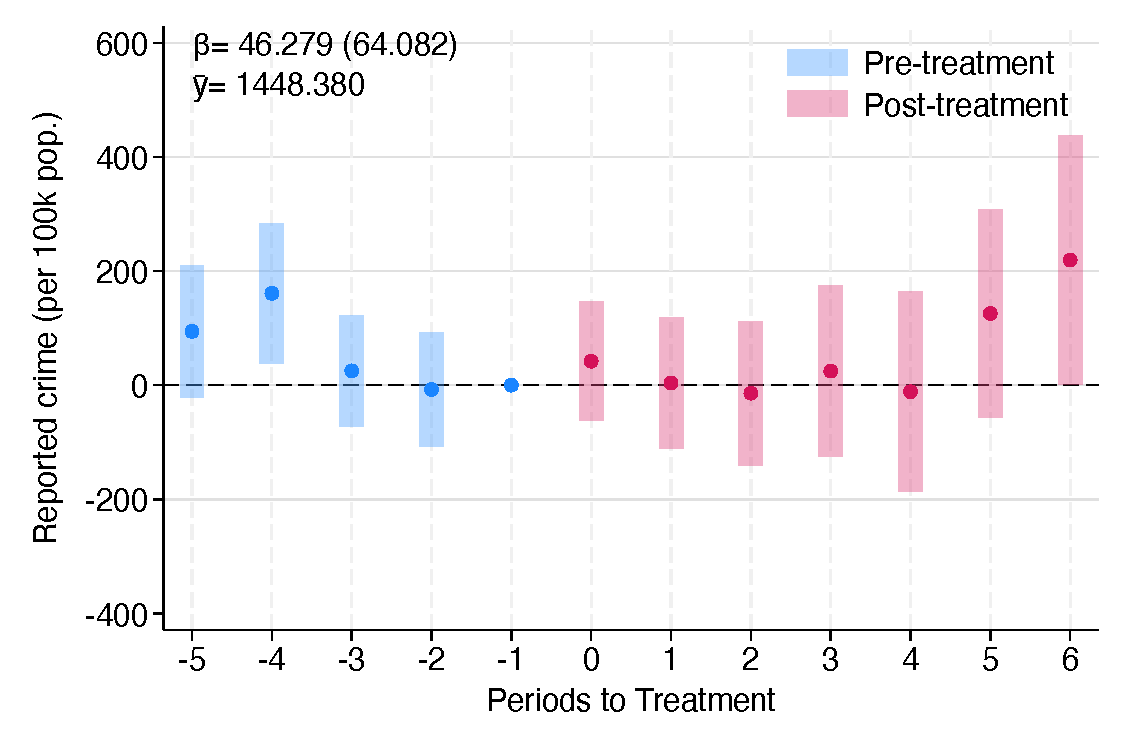
\includegraphics[width=0.98\textwidth]{../manuscript/Graphs/totalreportedcrime_allcomunas_neighbors.pdf}
        \caption{Spillovers on Reported crime}
    \end{subfigure}%
    ~ 
    \begin{subfigure}{0.495\textwidth}
    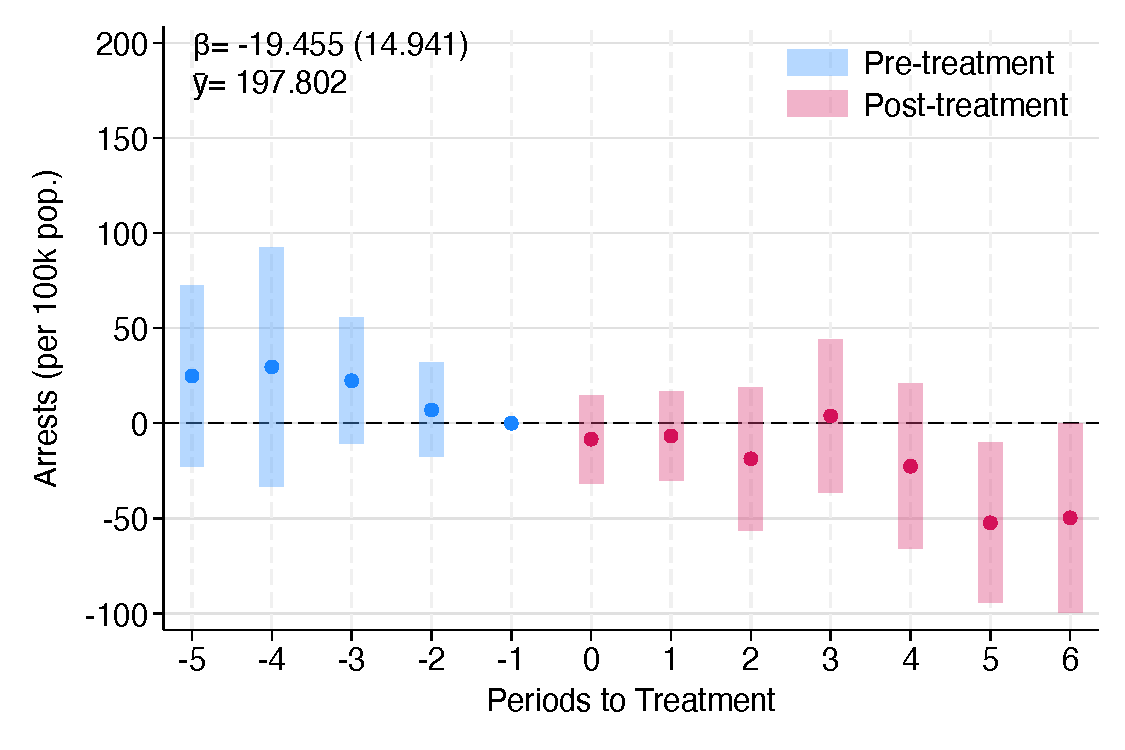
\includegraphics[width=0.98\textwidth]{../manuscript/Graphs/totalarrestscrime_allcomunas_neighbors.pdf}
        \caption{Spillovers on Arrests}
    \end{subfigure}
    \begin{subfigure}{0.495\textwidth}
        \centering
        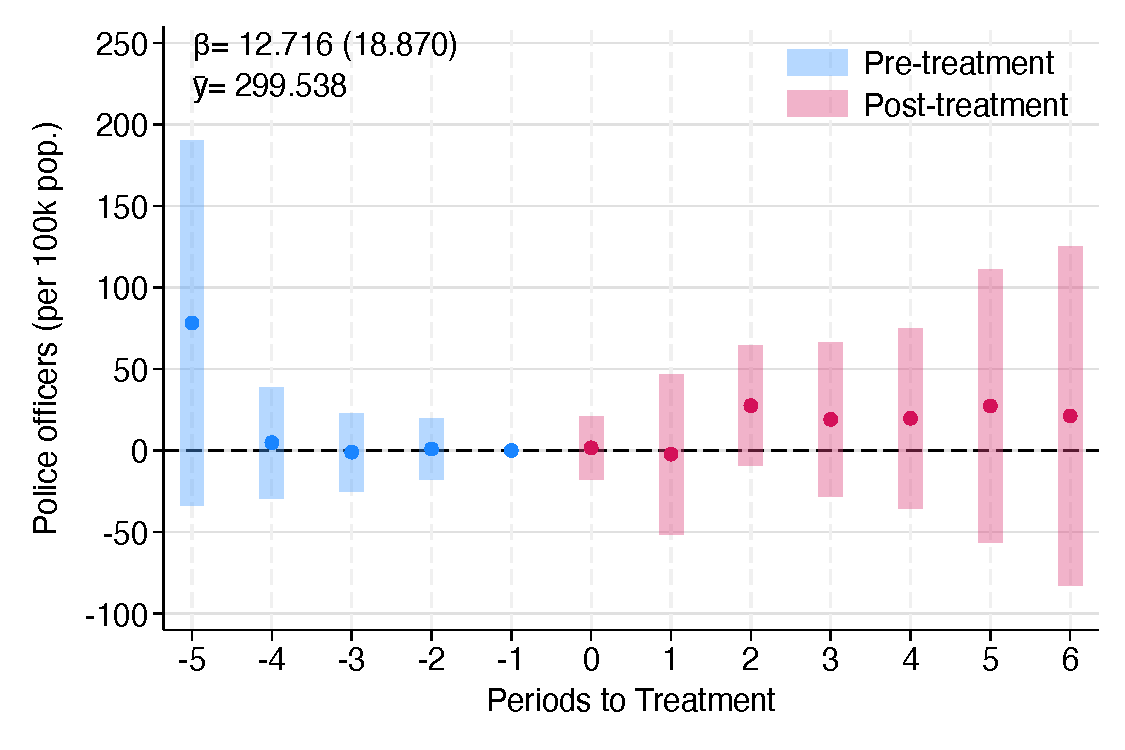
\includegraphics[width=0.98\textwidth]{../manuscript/Graphs/dotpc_allcomunas_neighbors.pdf}
        \caption{Spillovers on Police Officers}
    \end{subfigure}%
    ~ 
    \begin{subfigure}{0.495\textwidth}
    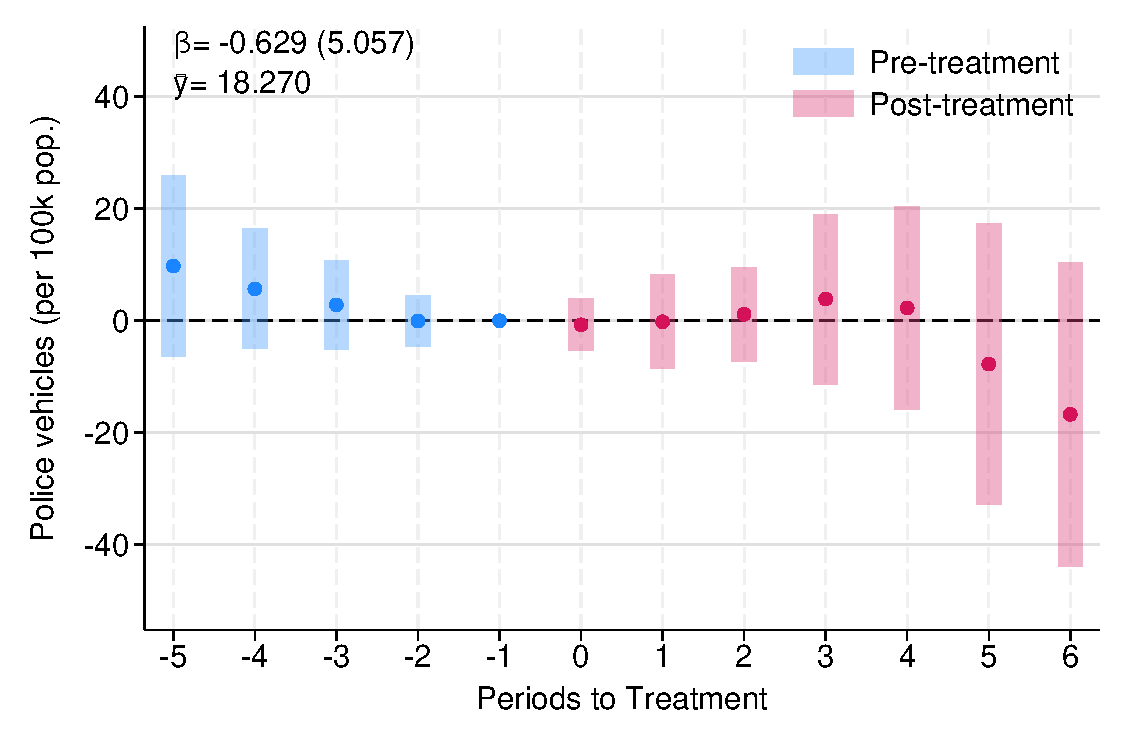
\includegraphics[width=0.98\textwidth]{../manuscript/Graphs/vehiclespc_allcomunas_neighbors.pdf}
        \caption{Spillovers on Patrol Vehicles}
    \end{subfigure}
    \begin{minipage}{0.9\textwidth}
    \footnotesize
    Notes: This figure reports the spillover effects of \emph{Plan Cuadrante} on the number of crimes reported to the police in the municipality per 100,000 inhabitants (panel a), the number of arrests in the municipality per 100,000 inhabitants (panel b), the number of police officers per 100,000 inhabitants (panel c), and the number of patrol vehicles per 100,000 inhabitants (panel d). Panels (a)--(d) include 2,859, 2,166, 1,144, and 1,942 observations respectively. Specifically, the figure shows the dynamic effects of the \emph{Plan Cuadrante} for neighbor municipalities which never introduced the program. The estimation is conducted using the procedure developed in \citet{Callaway} for difference-in-differences with staggered treatment adoption, using as the treatment introduction date the earliest date of a neighboring municipality. The dots in the figure represent the estimated coefficients and the bars behind them 95\% confidence intervals. Standard errors are clustered at the municipality level using the wild bootstrapping procedure. The pooled effect and the mean outcome before the introduction of the treatment for every outcome is also presented in each panel. 
    \end{minipage}
\end{figure}

\clearpage

\begin{figure}[h!]
    \centering
    \caption{Geographic Spillovers of \emph{Plan Cuadrante} for Neighbors of the ENUSC Municipalities (Administrative Outcomes)}
    \label{fig:figure_46ENUSC_spillovers_admin}
    \begin{subfigure}{0.495\textwidth}
        \centering
        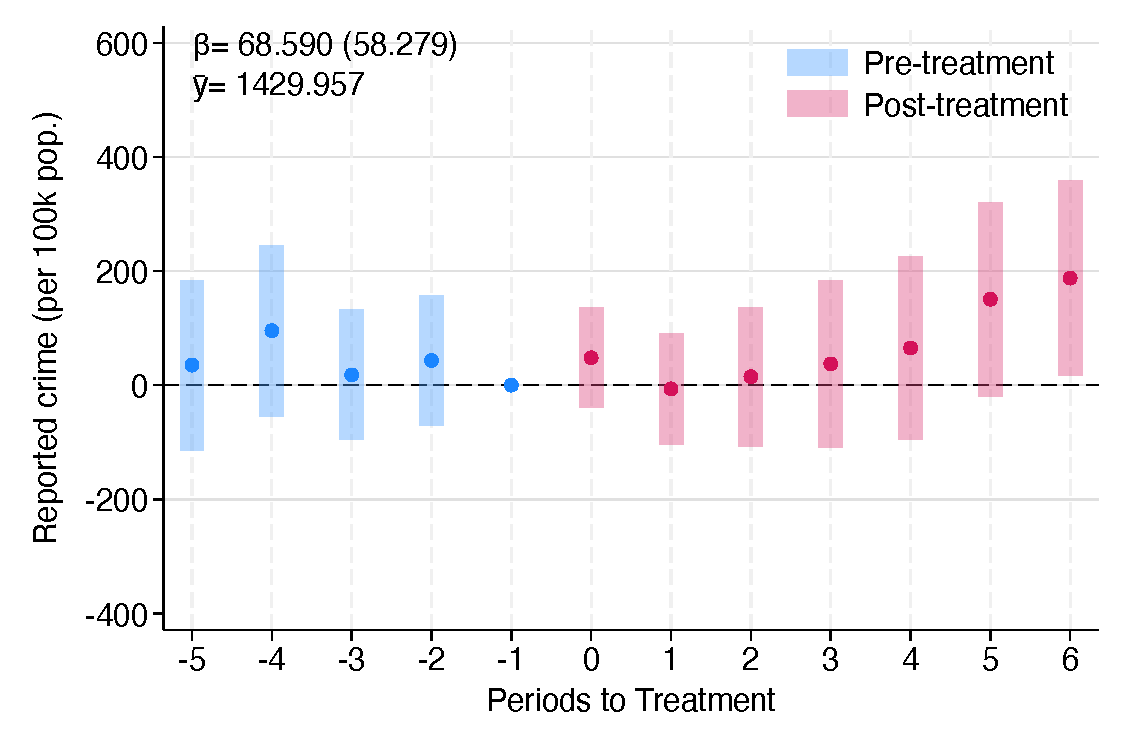
\includegraphics[width=0.98\textwidth]{../manuscript/Graphs/totalreportedcrime_enusc47_neighbors.pdf}
        \caption{Spillovers on Reported Crime}
    \end{subfigure}%
    ~
    \begin{subfigure}{0.495\textwidth}
        \centering
        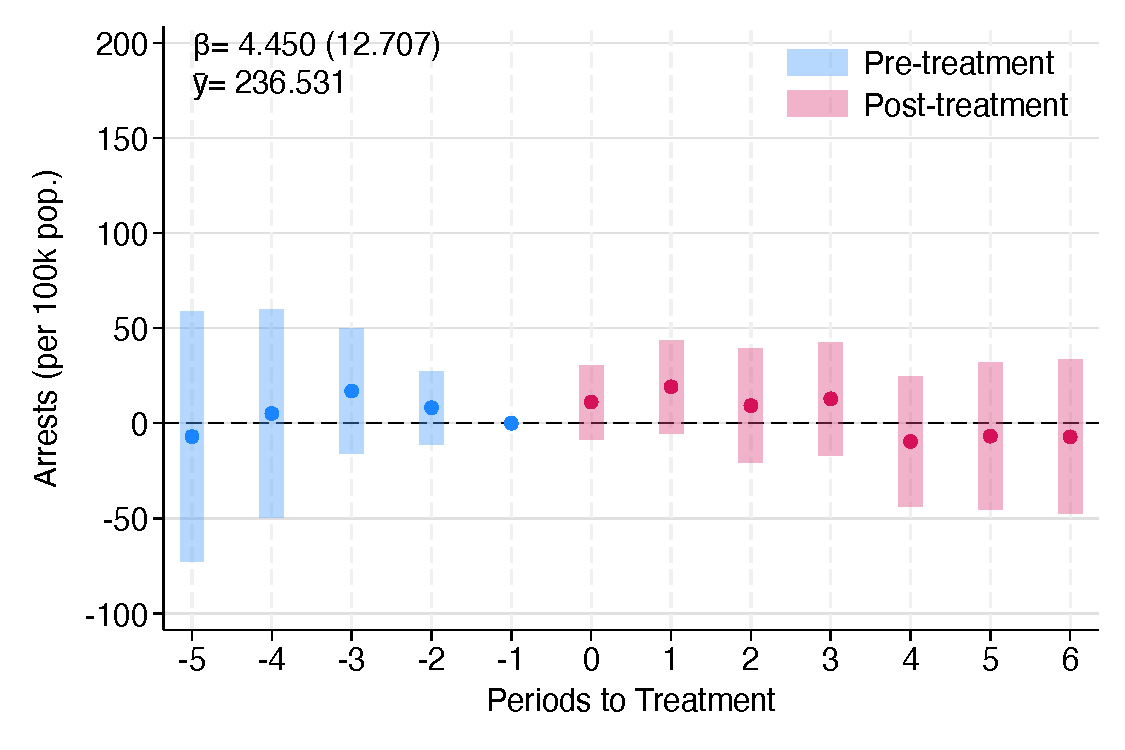
\includegraphics[width=0.98\textwidth]{../manuscript/Graphs/totalarrestscrime_enusc47_neighbors.pdf}
        \caption{Spillovers on Arrests}
    \end{subfigure}

    \vspace{0.5em}

    \begin{subfigure}{0.495\textwidth}
        \centering
        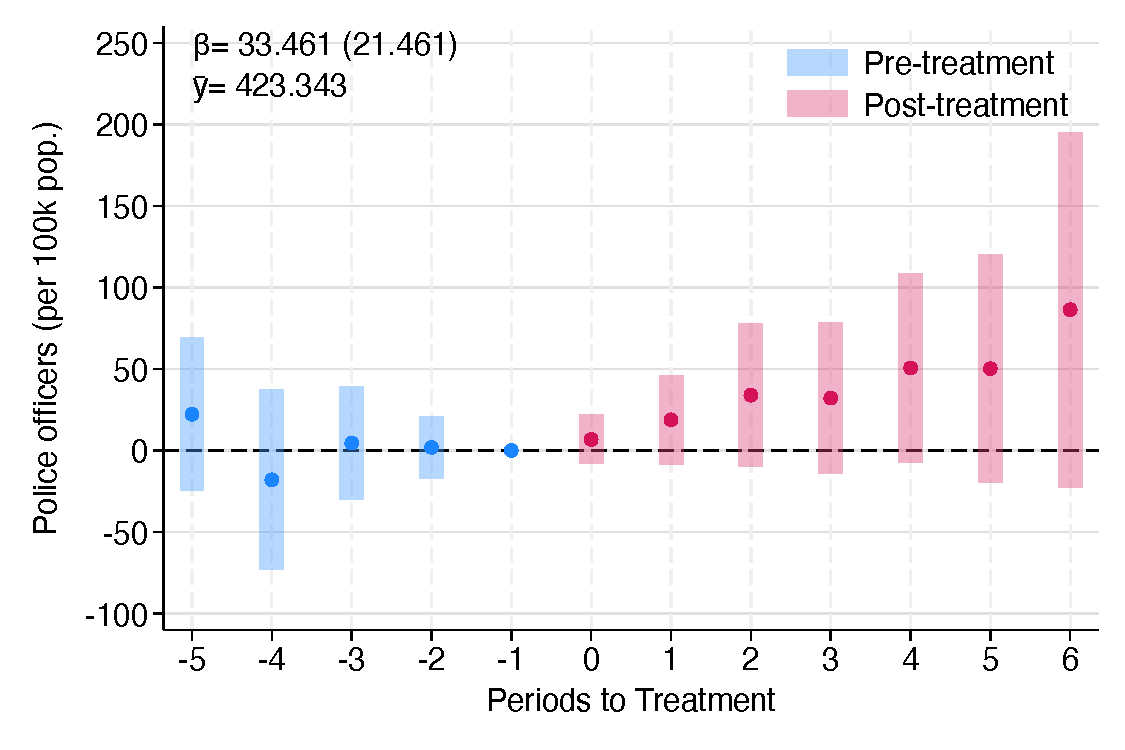
\includegraphics[width=0.98\textwidth]{../manuscript/Graphs/dotpc_enusc47_neighbors.pdf}
        \caption{Spillovers on Police Officers}
    \end{subfigure}%
    ~
    \begin{subfigure}{0.495\textwidth}
        \centering
        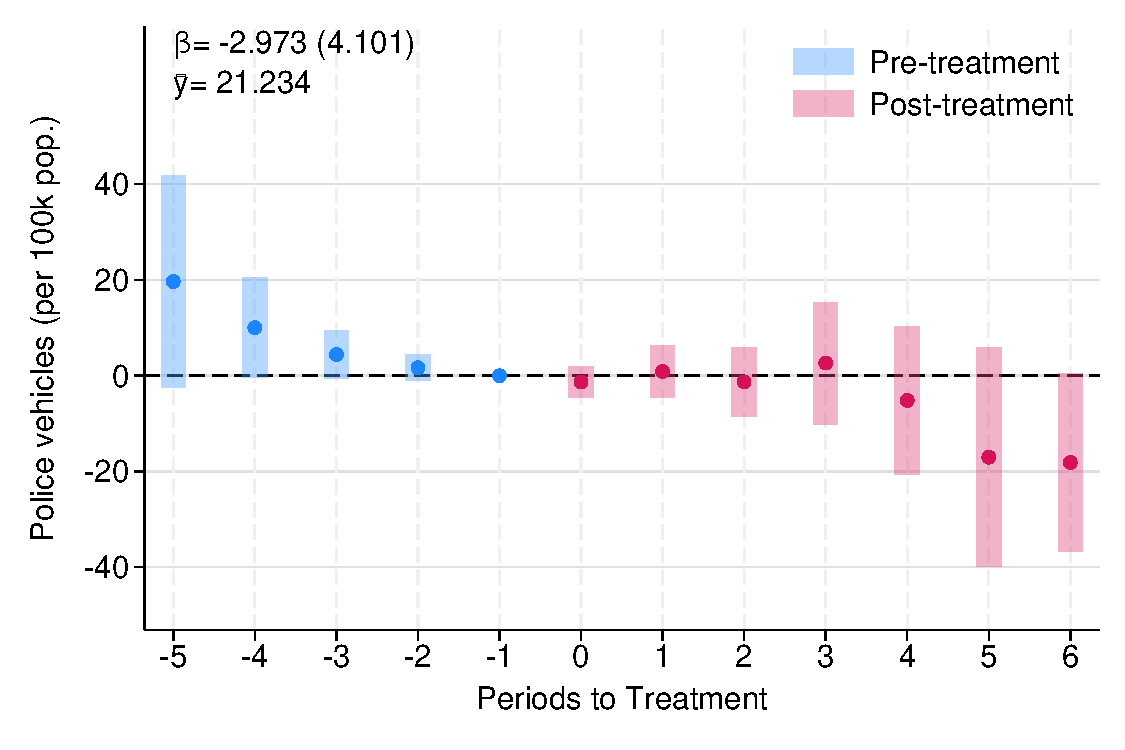
\includegraphics[width=0.98\textwidth]{../manuscript/Graphs/vehiclespc_enusc47_neighbors.pdf}
        \caption{Spillovers on Patrol Vehicles}
    \end{subfigure}

\begin{minipage}{\textwidth}
\footnotesize Notes: This figure reports the spillover effects of \emph{Plan Cuadrante} on the number of crimes reported to the police in the municipality per 100,000 inhabitants (panel a), on the number of arrests in the municipality per 100,000 inhabitants (panel b), on the number of police officers (panel c), and on the number of patrol vehicles (panel d). Specifically, the figure shows the dynamic effects of \emph{Plan Cuadrante} for neighboring never-treated municipalities to the 46 municipalities included in the ENUSC sample. The estimation is conducted using the procedure developed in \citet{Callaway} for difference-in-differences with staggered treatment adoption, using as the treatment introduction date the earliest date of a neighboring municipality. The dots in the figure represent the estimated coefficients and the bars behind them 95\% confidence intervals. Standard errors are clustered at the municipality level using the wild bootstrap procedure. The pooled effect and the mean outcome before the introduction of the treatment for each outcome are also presented in each panel.
\end{minipage}
\end{figure}


\begin{figure}[h!]
    \centering
    \caption{Geographic Spillovers of \emph{Plan Cuadrante} on ENUSC Survey Outcomes (Early- to Late-Adopting Municipalities)}
    \label{fig:figure_results_spillovers_enusc}
    \begin{subfigure}{0.495\textwidth}
        \centering
        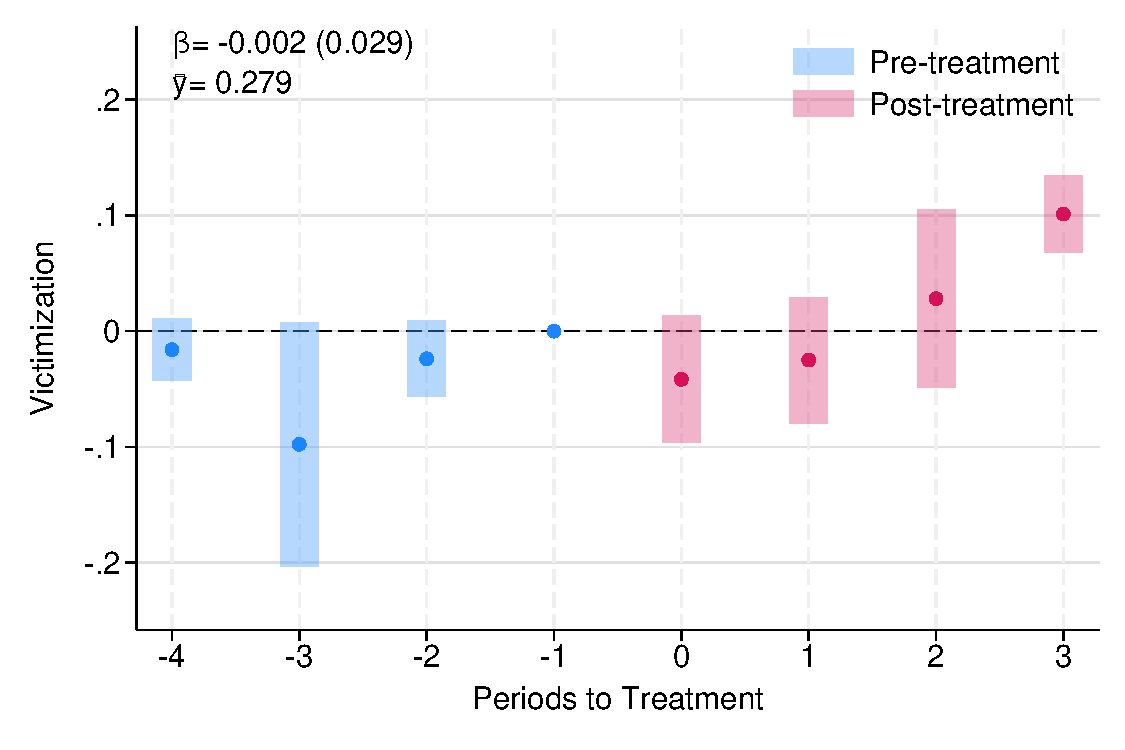
\includegraphics[width=0.98\textwidth]{../manuscript/Graphs/results_spillover_delitos.pdf}
        \caption{Spillovers on Victimization in last 12 months}
    \end{subfigure}%
    ~
    \begin{subfigure}{0.495\textwidth}
        \centering
        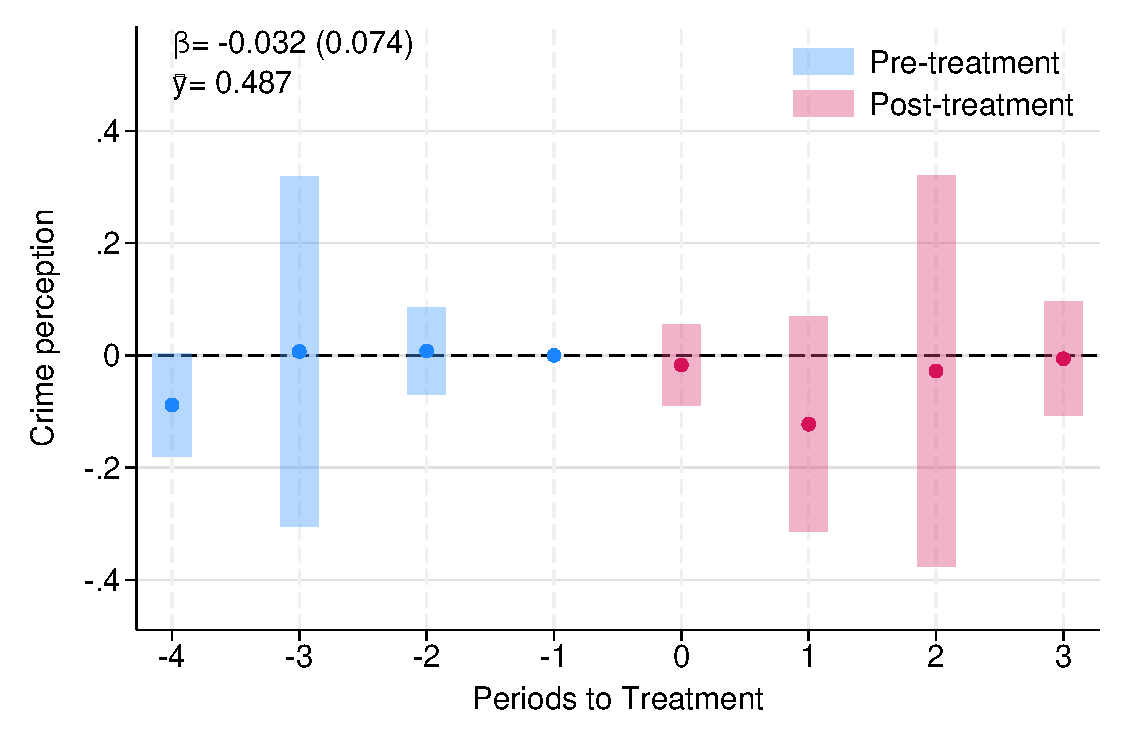
\includegraphics[width=0.98\textwidth]{../manuscript/Graphs/results_spillover_inseguridad_barrio1.pdf}
        \caption{Spillovers on Households reporting an increase in crime}
    \end{subfigure}
    \vspace{0.5em}
    \begin{subfigure}{0.495\textwidth}
        \centering
        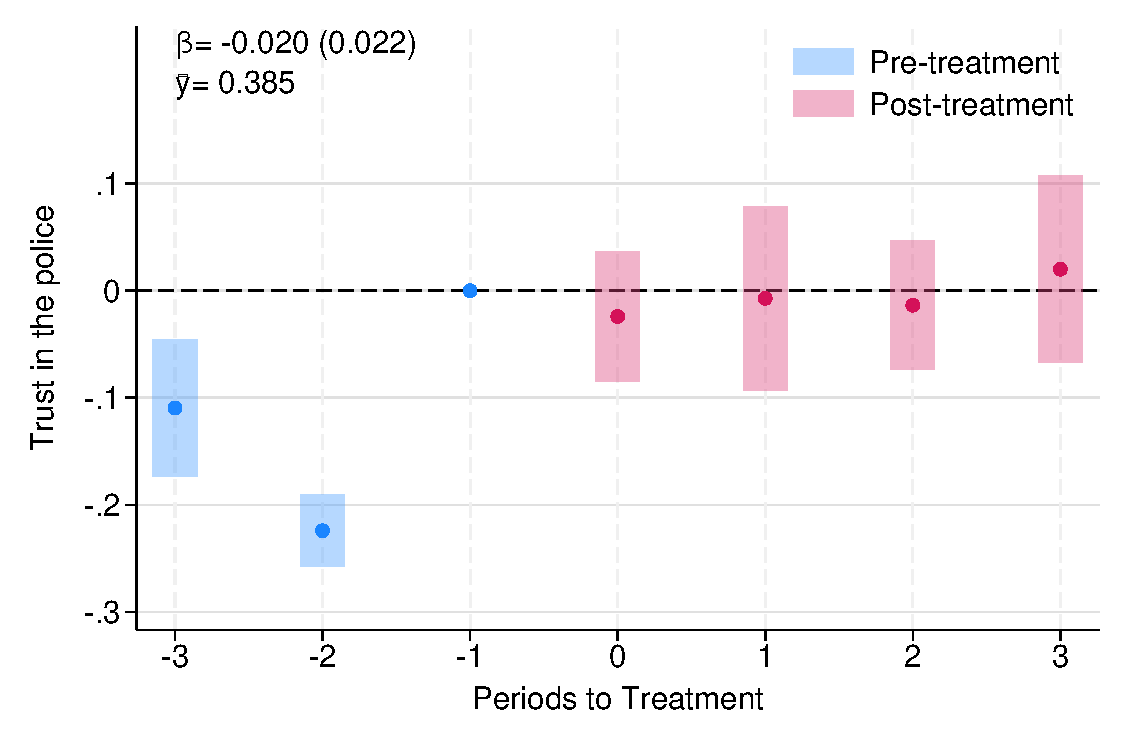
\includegraphics[width=0.98\textwidth]{../manuscript/Graphs/results_spillover_confianza_carabineros.pdf}
        \caption{Spillovers on Trust in the police}
    \end{subfigure}%
    ~
    \begin{subfigure}{0.495\textwidth}
        \centering
        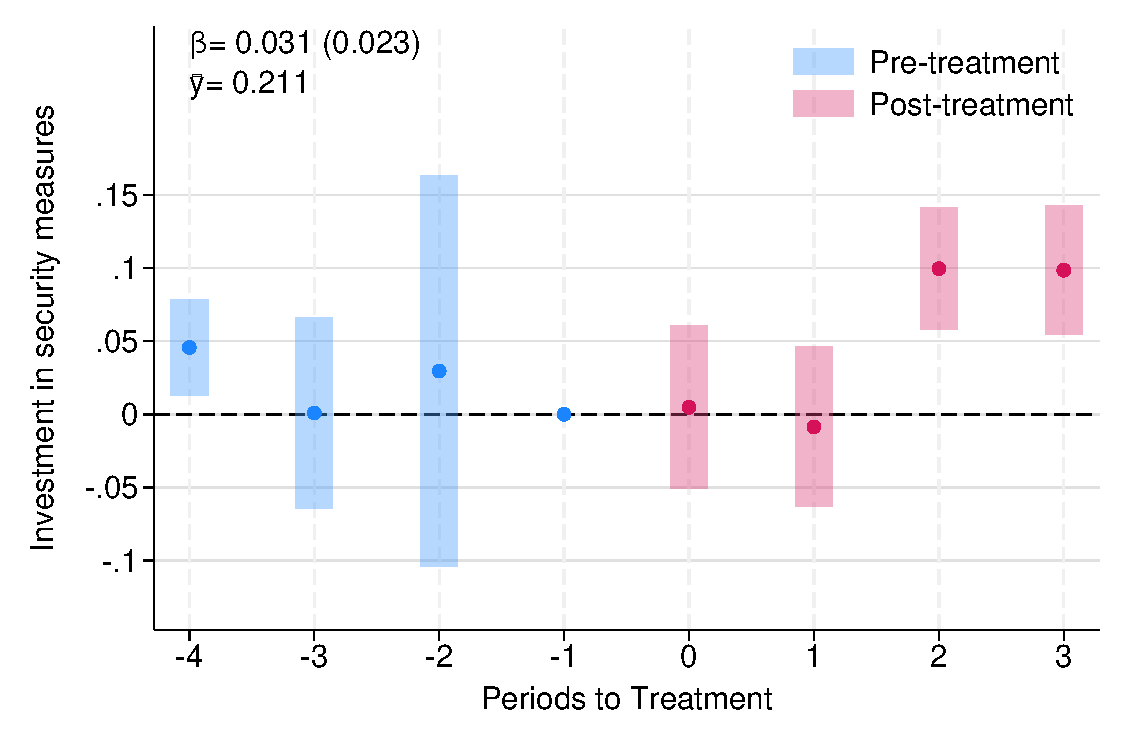
\includegraphics[width=0.98\textwidth]{../manuscript/Graphs/results_spillover_medidas_general_12.pdf}
        \caption{Spillovers on Households adopting security measures}
    \end{subfigure}
    \begin{minipage}{0.95\textwidth}
    \footnotesize
    Notes: This figure presents the geographic spillover effects of \emph{Plan Cuadrante} from early-adopting ENUSC municipalities on their late-adopting ENUSC neighbours, using the ENUSC sample. Panel (a) reports the effect of \emph{Plan Cuadrante} on the probability of household victimization in the last 12-months using the ENUSC survey. Panel (b) reports the effect on crime perception using the ENUSC survey. Panel (c) reports the effect on trust in the police using the ENUSC survey. Panel (d) reports the results on the probability of purchasing private security measures in the last twelve months using the ENUSC survey. The focal treated sample consists of six late-adopting ENUSC municipalities---Molina, Tocopilla, San Carlos, Padre Hurtado, Calera, and Limache---each assigned a spillover-onset date equal to the year its earliest-adopting ENUSC neighbour received \emph{Plan Cuadrante}: Curic\'o (2005) for Molina, Iquique (2005) for Tocopilla, Chill\'an (2007) for San Carlos, Pe\~naflor (2008) for Padre Hurtado, and Quillota (2008) for both Calera and Limache. Estimation is performed using the difference-in-differences estimator for staggered treatment adoption of \citet{Callaway}. The dots represent the estimated dynamic effects and the bars behind them denote 95\% confidence intervals. Standard errors are clustered at the municipality level. The pooled effect  and the mean of the outcome among municipalities with no treated neighbors are reported in each panel.
    \end{minipage}
\end{figure}


\clearpage
